Das  Kernst\"uck  dieser Arbeit  und  des  zugeh\"origen Softwaretools  stellt
die   so  genannte   ``Phasengang-Methode   zur  Reglerdimensionierung''   von
Jakob   Zellweger   dar~\cite{regelungstechnik:zellweger_short}. Diese   wurde
urspr\"unglich  als  vereinfachte  grafische  Methode  zur  Approximation  der
-20dB/Dek Methode erarbeitet und im Rahmen dieses Projektes in einem Java-Tool
automatisiert. Als  Vergleich   wertet  die  Software  ebenfalls   einige  der
g\"angigen Faustformeln aus.

Das Tool f\"uhrt grob vereinfacht folgende Schritte aus:
\begin{itemize}
    \item
        Bestimmung des  Frequenzgangs der Regelstrecke  aus Verz\"ogerungszeit
        $T_u$,     Anstiegszeit     $T_g$      und     Verst\"arkung     $K_s$
        (Abschnitt~\ref{subs:frequenzgang})
    \item
        Dimensionierung       des      Reglers       mittels      Faustformeln
        (Abschnitt~\ref{subs:faustformeln})
    \item
        Dimensionierung      des      Reglers     durch      Phasengangmethode
        (Abschnitte~\ref{subs:phasengang:pi} und~\ref{subs:phasengang:pid})
    \item
        Umrechung   der   Regler-Darstellung    zwischen   bodekonformer   und
        reglerkonformer Darstellung (Abschnitt~\ref{subs:bode_regler})
    \item
        Berechnung   der   Schrittantwort   des   geschlossenen   Regelkreises
        (Abschnitt~\ref{subs:geschlossen})
\end{itemize}

Im  folgenden   Kapitel  wird  auf   diese  Punkte  genauer   eingegangen  und
das  Vorgehen  anhand  eines  konkreten  Beispiels  rechnerisch  und  grafisch
erl\"autert. Die   Durchrechnung   der   Phasengangmethode   orientiert   sich
an   den   Rezepten,   welche   im   fachlichen   Teil   des   Pflichtenheftes
dieses    Projektes    zu    finden    sind~\cite{ref:pflichtenheft}. Genauere
Hintergrundinformationen    zur    Phasengangmethode     selbst    sind    dem
Skript~\cite{regelungstechnik:zellweger_short} zu entnehmen.

Das \"Uberschwingverhalten des Regelkreises soll  f\"ur dieses Projekt in drei
Stufen  berechnet werden. Verwendet  wird dazu  folgende Abstufung:  \todo{Ist
diese  Einteilung des  \"Uberschwingens noch  aktuell  oder wurde  das in  der
Auftragserweiterung angepasst?}

\begin{itemize}
    \item
        wenig \"Uberschwingen (ca. 0\%)
    \item
        mittleres \"Uberschwingen (ca. 16\%)
    \item
        starkes \"Uberschwingen (ca. 23\%)
\end{itemize}

\subsection{Grundlagen}

\subsection{Regelstrecke}
In der Regelungstechnik wird die zu regelnde Strecke als Regelstrecke bezeichnet. Die Regelstrecke wird durch ihr Zeitverhalten charakterisiert, welches den Aufwand und die Güte der Regelung bestimmt. Um das Zeitverhalten zu beschreiben verwendet man die Sprungantwort, welche zeigt, wie die Regelgrösse auf Stellgrössenänderung reagiert. Mit der entstehenden Regelgrösse werden verschiedene Regelstrecken unterschieden:
\begin{itemize}   
 \item  P-Regelstrecke
 \item I-Regelstrecke
 \item    Strecken mit einer Totzeit
 \item Strecken mit Energiespeicher
\end{itemize}

Dieses Projekt beschäftigt sich mit  den PTn-Strecken, welche eine Kombination aus einer Strecke mit proportionalen Verhalten und einer mit Totzeit sowie der Angabe der  Ordnung n der Strecke.

\subsubsection*{P-Regelstrecke}
Bei der Regelstrecke mit proportionalem Verhalten folgt die Regelstrecke proportional der Stellgrösse ohne Verzögerung. Dies kommt in der Praxis nicht vor, da immer eine Verzögerung vorhanden ist. Ist diese jedoch sehr klein spricht man von einer P-Strecke. Das Verhalten der Strecke ist in seinem Blockschaltbild (Abb.\ref {fig:PStrecke}) symbolisch dargestellt. Der Proportionalitätsfaktor wird mit $K_p$ abgekürzt. Wird $K_p<1$ wirkt $K_p$ nicht mehr verstärkend sondern abschwächend.\\

\begin{figure}[h!, width=\pagewidth]
\begin{center}
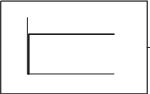
\includegraphics[width=0.5\textwidth]{PStrecke}
\caption{Blockschaltbild von P-Strecke}
\label{fig:PStrecke}
\end{center}
\end{figure}


\subsubsection*{Strecken mit Totzeit}
Ändert sich die Stellgrösse, wirkt sich diese Änderung bei einer Strecke mit Totzeit erst nach einer gewissen Zeit auf die Regelgrösse aus. Mit $T_t$ wird das Mass der Totzeit gekennzeichnet. 
Totzeiten verursachen schnell Schwingungen, da sich die Stellgrösseänderung zeitverzögert auf die Regelgrösse auswirkt. Die Schwingungen entstehen wenn sich die Stellgrösse und die Regelgrösse periodisch ändern.

\begin{figure}[h!, width=\pagewidth]
\begin{center}
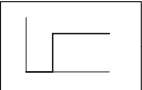
\includegraphics[width=0.5\textwidth]{images/TotZeit}
\caption{Blockschaltbild von Strecke mit Totzeit}
\label{fig:TotZeit}
\end{center}
\end{figure}


\subsubsection*{I-Regelstrecke}
Die I-Regelstrecke antwortet auf eine Stellgrössenänderung mit einer fortwährenden 
Änderung in steigende oder fallende Richtung. Die Begrenzung dieses Vorganges ist mit den systemgegeben Schranken gegeben. Die Integrierzeit $T_i$ ist ein Mass für die Anstiegsgeschwindigkeit der Regelgrösse und das Blockschaltbild (Abb. \ref{fig:IStrecke}) zeigt das Verhalten sinnbildlich.
\begin{figure}[h!, width=\pagewidth]
\begin{center}
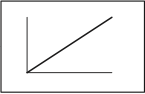
\includegraphics[width=0.75\textwidth]{images/IStrecke}
\caption{Blockschaltbild von I-Strecke}
\label{fig:IStrecke}
\end{center}
\end{figure}


\subsection{Regler}
Die Aufgabe eines Reglers besteht die zu regelnde Strecke mit einem Stellsignal so zu beeinflussen, dass der Wert der Regelgrösse gleich dem Wert der Führungsgrösse entspricht. Der Regler besteht aus einem Vergleichsglied, welches die Reglerdifferenz aus der Differenz zwischen Führungs- und Reglergrösse bildet und dem Reglerglied. Das Reglerglied erzeugt aus der Reglerdifferenz die Stellgrösse.\\
Es wird zwischen P-, I- und D-Regler unterschieden.
In diesem Projekt werden die PI- und PID-Regler, welche Kombinationen der oben genannten Regler sind, behandelt.\\

\subsubsection{PI-Regler}
Der PI-Regler besteht aus einer Parallelschaltung von einem P- und einem I-Regler (Abb.\ref{fig:PIRegler}). Durch diese Kombination werden die Nachteile beider Regler aufgehoben und die Vorteile (schnell, stabil) hervorgehoben. Sein Verhalten wird bildlich in dem Blockschaltbild in Abbildung \ref{fig:PIRegler2}.\\

\begin{figure}[h!, width=\pagewidth]
\begin{center}
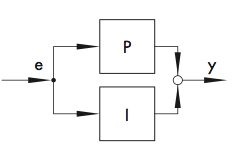
\includegraphics[width=0.5\textwidth]{images/PIRegler1}
\caption{Parallelschlatung von P-Regler und I-Regler}
\label{fig:PIRegler1}
\end{center}
\end{figure}

\begin{figure}[h!, width=\pagewidth]
\begin{center}
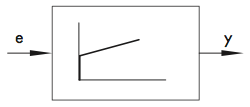
\includegraphics[width=0.75\textwidth]{images/PIRegler2}
\caption{Blockschaltbild von PI-Regler}
\label{fig:PIRegler2}
\end{center}
\end{figure}


\subsubsection{PID-Regler}
Wird dem PI-Regler ein D-Anteil parallel geschaltet (Abb. \ref{fig:PRDRegler}), entsteht der PID-Regler. Der PID-Regler ist ein sehr oft verwendeter Regler, da durch den D-Anteil die Regelgrösse rascher den Sollwert erreicht und der Einschwingvorgang schneller abgeschlossen ist. Das Blockschaltbild zeigt dieses Verhalten (Abb.\ref{fig:PIDRegler2}) figürlich. Der PID-Regler ist geeignet für Strecken höheren Ordnungen, welche möglichst schnell und ohne bleibende Regelabweichung geregelt werden müssen.

\begin{figure}[h!, width=\pagewidth]
\begin{center}
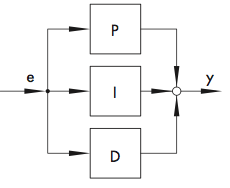
\includegraphics[width=0.75\textwidth]{images/PRDRegler1}
\caption{Parallelschaltung von P-, I-, und D-Regler}
\label{fig:PRDRegler1}
\end{center}
\end{figure}

\begin{figure}[h!, width=\pagewidth]
\begin{center}
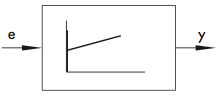
\includegraphics[width=0.75\textwidth]{images/PIDRegler2}
\caption{Personalkosten}
\label{fig:PIDRegler2}
\end{center}
\end{figure}


\subsubsection{Die Steuerung}

Unter einer Steuerung versteht man eine offen Wirkungskette wie in Abbildung \ref{fig:}, dass heisst die Wirkglieder sind kettenähnlich aufgereiht und besitzen keine Rückkopplung. Die Steuerkette wird genau für eine Steuerung ausgelegt und kann nur einer Störgrösseart entgegenwirken. Ohne die Rückkopplung wird das Ausgangsignal nicht mit dem Eingangssignal verglichen und es können keine Korrekturen vorgenommen werden.

\subsubsection{Der geschlossene Regelkreis}
Die Aufgabe eines geschlossenen Regelkreises (Abbildung \ref{fig:geschlossenerRegelkreis}) ist es, einen vorgegeben Sollwert zu erreichen und diesen
auch bei St\"orungen aufrecht zu erhalten. Dabei sollen die unten genannten
dynamischen Anforderungen eingehalten werden, damit die Stabilit\"at des
Regelsystems garantiert ist. Die wichtigste Bedingung f\"ur die Schrittantwort
ein geschlossenen Regelkreis heisst, dass der Regelfehler, die Differenz
zwischen Ist- und Sollwert, gleich Null oder m\"oglichst klein ist.\\


\begin{figure}[!h!, width=\pagewidth]
\begin{center}
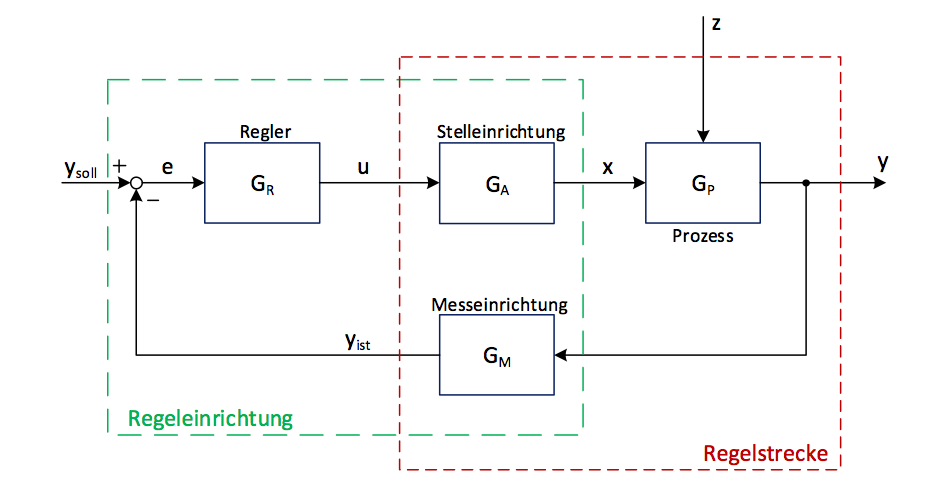
\includegraphics[width=0.5\textwidth]{images/geschlRegelkreis}
\caption{Geschlossener Regelkreis}
\label{fig:geschlossenerRegelkreis}
\end{center}
\end{figure}

%Name Bild Struktur eines allgemeinen Regelkreises
\begin{itemize}
\item
$y_soll$ bezeichnet den Sollwert der Regelgr\"osse.
\item
$e$ Regelabweichung (Regelfehler)
\item
$u$ Steuergr\"osse
\item
$x$ Stellgr\"osse
\item
$y$ Regelgr\"osse
\item
$z$ St\"orgr\"ossen werden in diesem Projekt nicht berücksichtigt
\item
$y_ist$ ist der Ist-Wert der Regelgr\"osse und wird auch als die
Schrittantwort des Regelkreises bezeichnet.
\end{itemize}


Grunds\"atzlich k\"onnen f\"unf Anforderungen f\"ur einen geschlossenen
Regelkreis und deren Schrittantworten zusammengefasst werden:\\
\begin{enumerate}
\item Der Regelkreis muss stabil sein:\\
F\"ur das Regelsystem heisst stabil, dass es in seinen
Gleichgewichtszustand zur\"uckgef\"uhrt werden kann.
\item
Der Regelkreis muss gen\"ugend ged\"ampft sein.
\item
Der Regelkreis muss eine bestimmte station\"are Genauigkeit
aufweisen: \\Das bedeutet, der Regelfehler e(t) soll f\"ur t-> oo
gegen Null gehen. 
\item
Der Regelkreis muss hinreichend schnell sein: 
Ist die D\"ampfung zu stark oder zu schwach, braucht der
Einschwingvorgang mehr Zeit. Hierbei muss darauf geachtet werden, dass
die spezifischen Anforderungen an das Regelsystem eingehalten werden.
\item
Der Regelkreis muss robust sein: Der Regelkreis muss so ausgelegt
werden, dass das Regelsystem auch im schlimmsten Fall (je nach
Regelsystem situationsabh\"angig) in der Lage ist, das System zur\"uck
in den stabilen Zustand (vgl. 1.) zu regeln.


\subsubsection{Die Schrittantwort des geschlossenen Regelkreises}
\todo{Bild Schrittantworten passend zu Aufzählung unten}

Als Schrittantwort eines geschlossenen Regelkreises wird das Ausgangssignal y(t) bezeichnet. Im Zusammenhang mit den Anforderungen an den geschlossenen Regelkreis, werden an die Schrittantwort folgende Forderungen gestellt:
\begin{enumerate}
\item
Die Schrittantwort eines stabilen Regelkreises darf nach dem Erreichen
des eingeschwungenen Zustand kein erneutes \"Uberschwingen auftreten.

\item
Die D\"ampfung der
Schrittantwort soll so stark sein, dass der eingeschwungene Zustand
m\"oglichst rasch erreicht wird ohne dass das \"Uberschwingen des
Systems zu stark wird.
\item Die Schrittantwort muss für ein t->oo gleich $y_soll$ sein.
\item Die Schnelligkeit des
Einschwingvorganges der Schrittantwort ist stark von der D\"ampfung
abh\"angig. Wenn diese zu stark oder zu schwach ist, ist der Regelkreis zu langsam.
\end{enumerate}

\todo{Abschnitt verfassen}

\clearpage
\subsection{Frequenzgang der Regelstrecke}
\label{subs:frequenzgang}
Als  Ausgangspunkt  der  Reglerdimensionierung dient  die  Schrittantwort  der
Strecke. Durch  Einzeichnen  der Wendetangente~\footnotemark[1]  ergeben  sich
Schnittpunkte  der  Wendetangente mit  der  Zeitachse  $[T_u,0]$ und  mit  dem
Zielwert  $[T_g+T_g,1]$.  Es  k\"onnen nun  also die  Verz\"ogerungszeit $T_u$
und die  Anstiegszeit $T_g$  aus aus  Abbildung~\ref{fig:plant_step} abgelesen
werden.

\footnotetext[1]{%
    Die Wendetangante ist die Tangente an den Wendepunkt in der Anstiegs-Phase
    der Schrittantwort.
}

Wir werden in diesem Bericht folgende Strecke als Beispiel nehmen:
\begin{figure}[h! width=\pagewidth]
    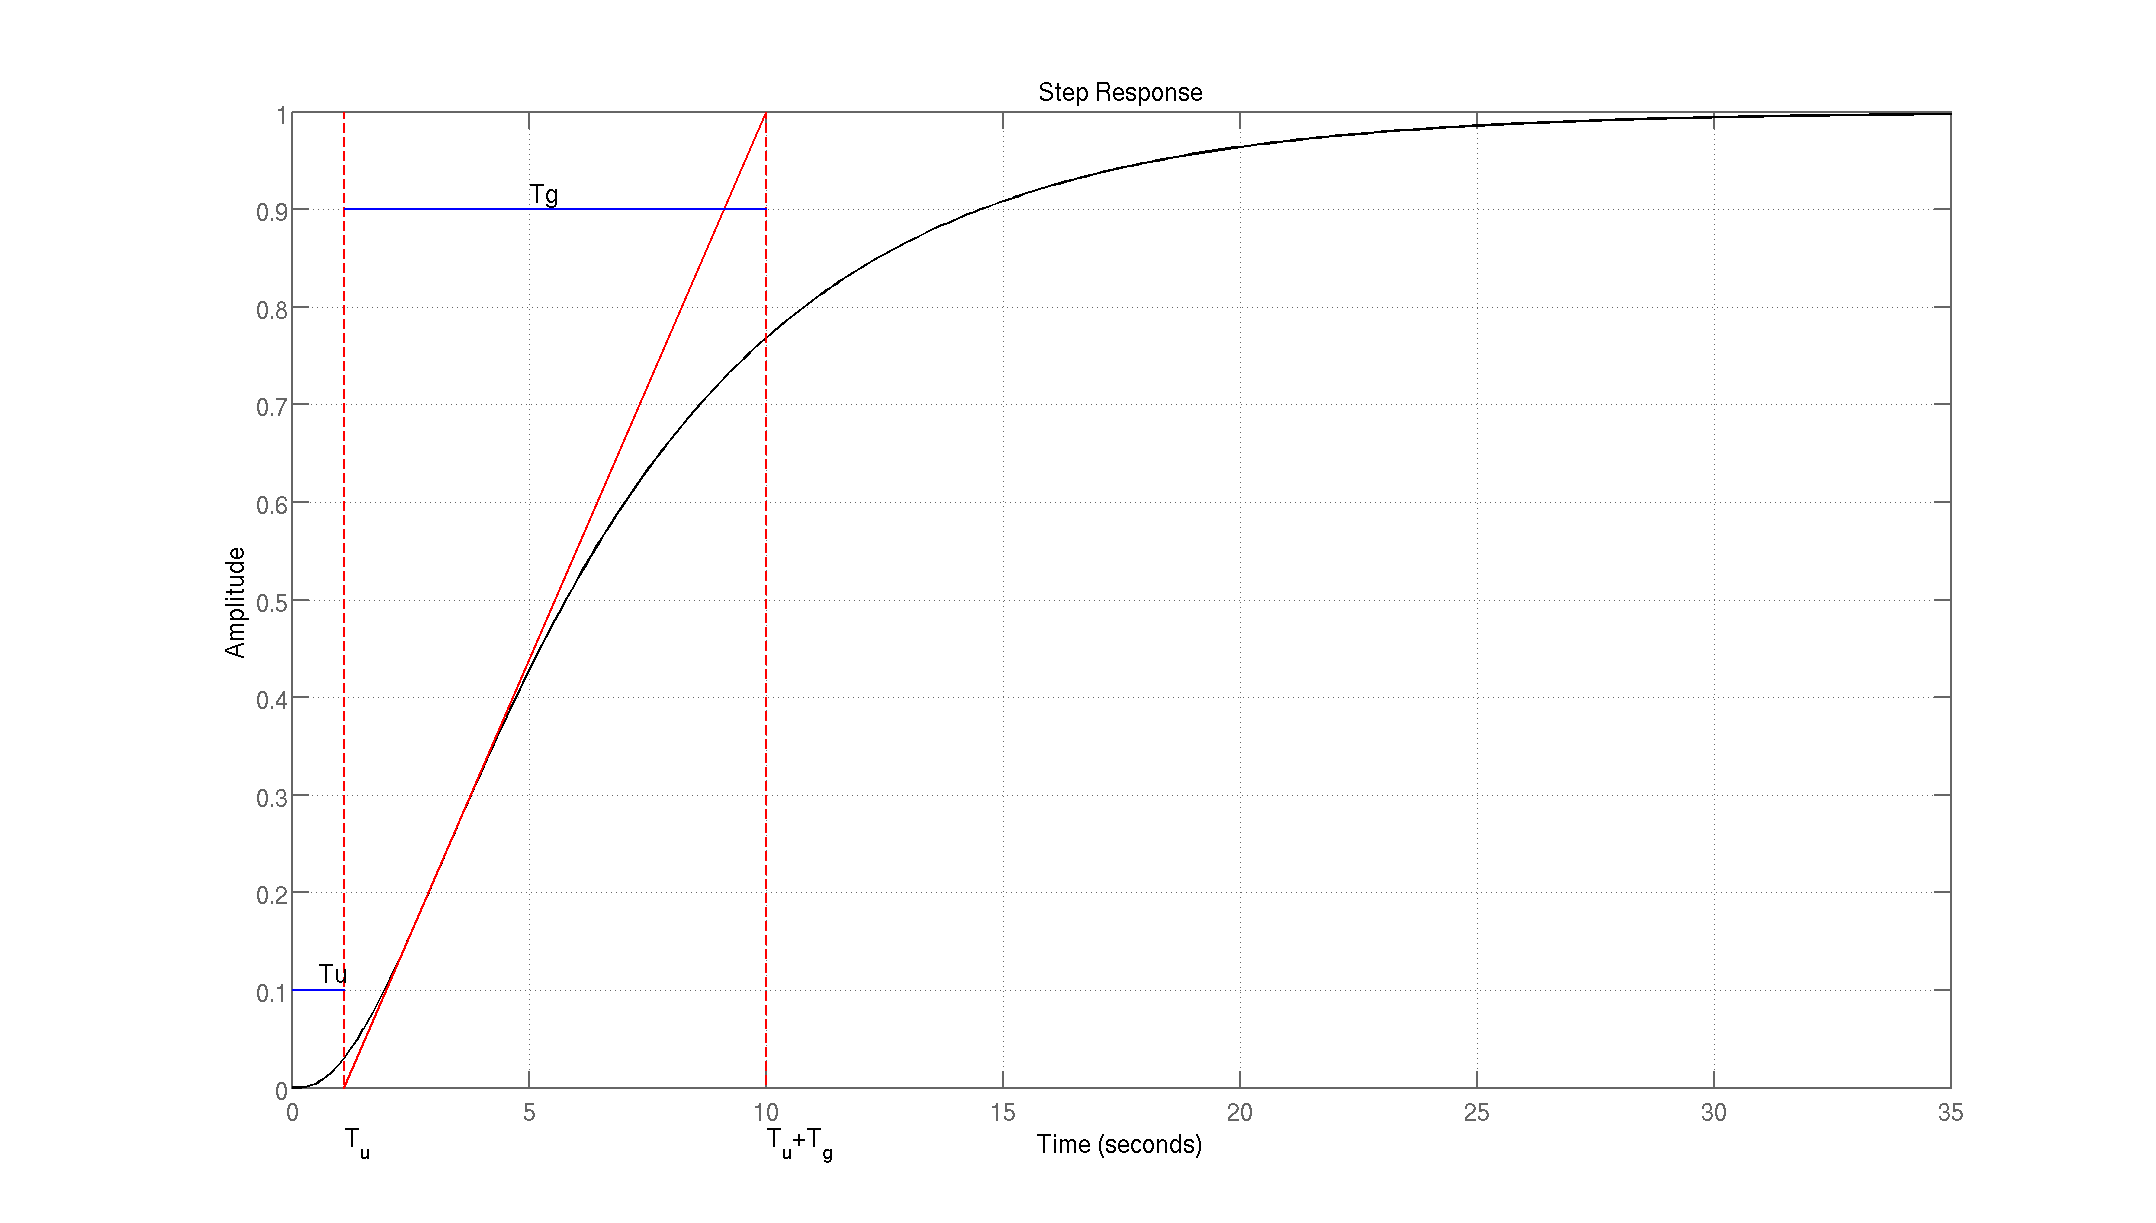
\includegraphics[width=\textwidth]{images/streckeSchrittantwort.png}
    \caption{%
    Schrittantwort der  Beispielstrecke (schwarz), Wendetangende  (rot), $T_u$
    und $T_g$ (blau)
    }
    \label{fig:plant_step}
\end{figure}

Ausmessen der Schrittantwort ergibt:
\begin{itemize}
    \item
        $K_s = 2$~\footnotemark[2]
    \item
        $T_u = \SI{1.1}{\second}$
    \item
        $T_g = \SI{8.9}{\second}$
\end{itemize}

\footnotetext[2]{%
    Abbildung~\ref{fig:plant_step}  ist  auf  1  normiert,  die  Verst\"arkung
    unserer  Beispielstrecke   betr\"agt  $2$.    An  den  Werten   f\"ur  die
    Verz\"ogerungs-  und Anstiegszeit  oder  am  Ausmessen der  Schrittantwort
    \"andert sich dadurch nichts
}

Der  geschlossene   Regelkreis  soll  schlussendlich  maximal   etwa  $16.3\%$
\"uberschwingen.

Da die Reglerdimensionierung mit der Phasengangmethode vom \emph{Frequenzgang}
einer   Strecke  ausgeht   und   nicht  von   deren  Schrittantwort,   besteht
der   n\"achste   Schritt    nun   darin,   aus   den    obigen   Werten   den
Frequenzgang   der   Strecke   zu   bestimmen. Dies   erledigt   die   Methode
\code{p\_sani}\footnotemark[3],    welche   uns    die    Werte   f\"ur    die
\"Ubertragungsfunktion  der  Strecke  liefert.
  In unserem  Fall ergibt
dies folgendes Polynom:

\footnotetext[3]{%
    Die  Methode  \code{p\_sani}  wurde  zu  Beginn  des  Projektes  in  einer
    Matlab-Implementation  zur Verf\"ugung  gestellt  und anschliessend  f\"ur
    unser Tool in Java \"ubersetzt.

    Sie kann aus der Verz\"ogerungszeit, der Anstiegszeit und der Verst\"arkung
    der Strecke ein Polynom f\"ur deren \"Ubertragungsfunktion vom Grad 1 bis 8
    ausrechnen.

    Als Eingabeparameter werden  die Werte $T_u$, $T_g$  und $K_s$ ben\"otigt,
    als R\"uckgabewert erh\"alt  man ein Array mit den Zeiten  $T_i$ f\"ur die
    Nenner der Faktoren des Polynoms (siehe Gleichung~\ref{eq:transfer:plant}).
}

\begin{gather} \label{eq:transfer:plant}
    \begin{split}
        H_s (s) & = K_s
                  \cdot \frac{1}{1 + s \cdot T_1}
                  \cdot \frac{1}{1 + s \cdot T_2}
                  \cdot \frac{1}{1 + s \cdot T_2}                     \\
                & = 2
                  \cdot \frac{1}{1 + s \cdot \SI{0.4134}{\second}}
                  \cdot \frac{1}{1 + s \cdot \SI{1.4894}{\second}}
                  \cdot \frac{1}{1 + s \cdot \SI{5.3655}{\second}}
    \end{split}
\end{gather}

Mit einem  geeigneten Tool  kann man sich  den dazugeh\"origen  Plot erstellen
lassen.

\begin{figure}[h! width=\pagewidth]
    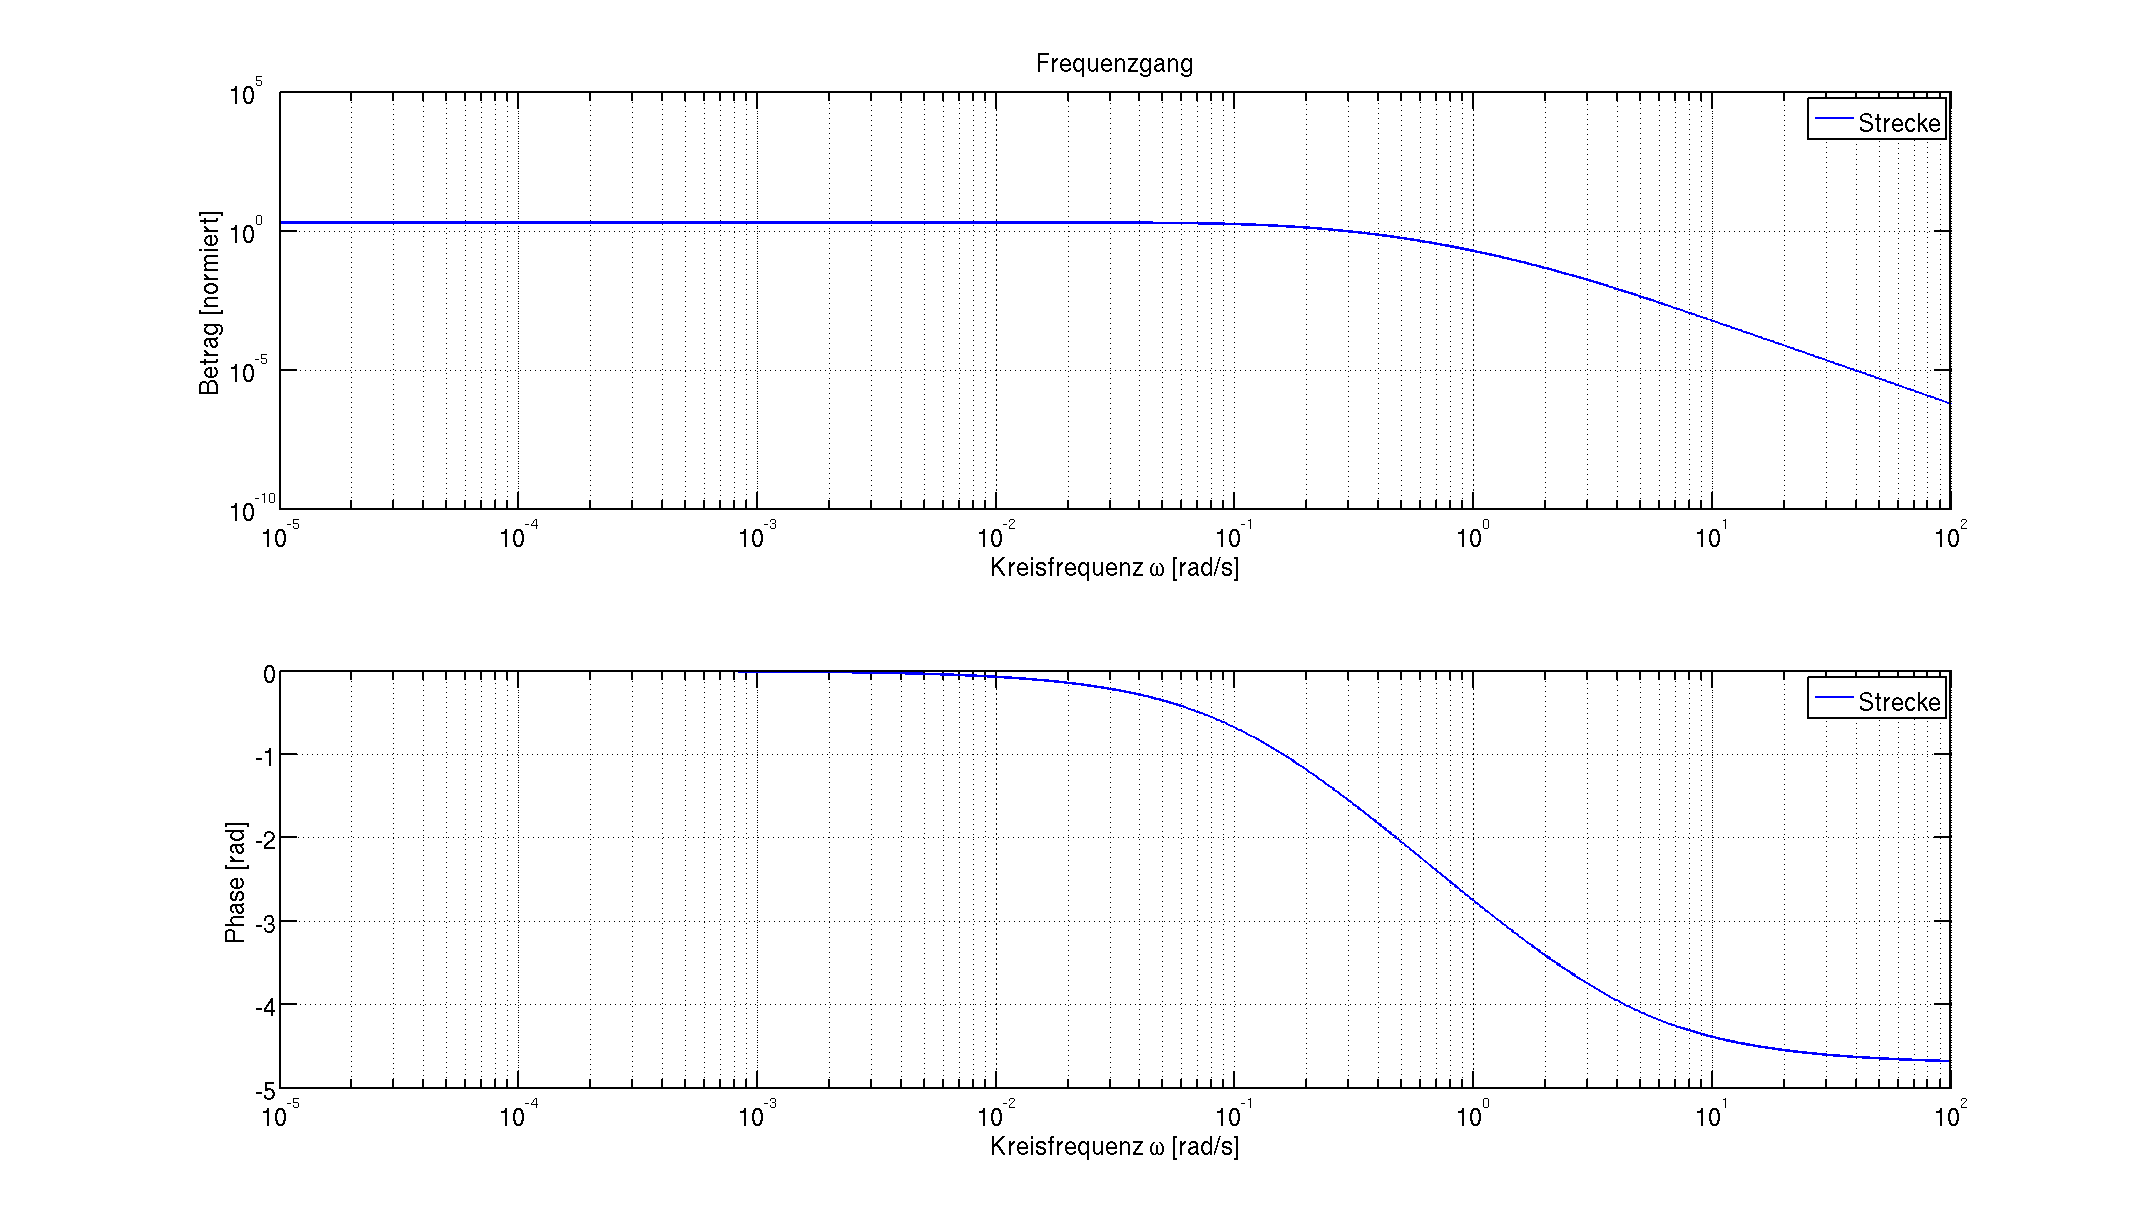
\includegraphics[width=\textwidth]{images/streckeFrequenzgang.png}
    \caption{%
        Frequenzgang der Strecke%
    }
    \label{fig:plant_freq}
\end{figure}

Somit  ist  der Frequenzgang  der  Strecke  bekannt  und  man kann  mit  einer
geeigneten Methode den Regler dimensionieren.


\subsection{Reglerdimensionierung mittels Faustformeln}
\label{subs:faustformeln}
Im   Praxiseinsatz  stehen   f\"ur   die  Dimensieung   der  Regler   einfache
Berechnungsformeln f\"ur die Einstellwerte der  Regler anhand von $T_u$, $T_g$
und $K_s$ zur Verf\"ugung.

Einige   dieser  Faustformeln   werden  in   der  Applikation   zum  Vergleich
mitberechnet. Die    dazugeh\"origen    Berechnungen    sind    der    Tabelle
\ref{tab:faustformeln} zu entnehmen.

\begin{longtable}{p{50mm}rrrrr}
    \toprule

    %\multicolumn{3}{l}{\large{\textsc{Auftragsanalyse und Hintergrundinformationen}}} \\

    Faustformel
    &
    \multicolumn{2}{l}{PI-Regler}
    &
    \multicolumn{2}{l}{PID-T1-Regler}
    \\

    &
    $T_n$
    &
    $K_p$
    &
    $T_n$
    &
    $T_v$
    &
    $K_p$
    \\

    \midrule

    \endhead
    \endfoot
    \endlastfoot

    % CONTENT HERE ---------------------------------------------------------- %

    \pbox{45mm}{Chiens, Hrones, Reswick \\ \small{\textbf{(0\% \"Uberschwingen)}} \\ \cite{ref:chiens_tsn}, \cite{ref:chiens_wiki}}
    &
    $1.2\cdot T_g$
    &
    $\frac{0.35}{K_s} \cdot \frac{T_g}{T_u}$
    &
    $T_g$
    &
    $0.5\cdot T_u$
    &
    $ \frac{0.6}{K_s} \cdot \frac{T_g}{T_u} $
    \\

    \addlinespace[1em]

    \pbox{45mm}{Chiens, Hrones, Reswick \small{\textbf{(20\% \"Uberschwingen)}} \\ \cite{ref:chiens_tsn}, \cite{ref:chiens_wiki}}
    &
    $T_g$
    &
    $\frac{0.6}{K_s} \cdot \frac{T_g}{T_u}$
    &
    $1.35\cdot T_g$
    &
    $0.47 \cdot T_u$
    &
    $ \frac{0.95}{K_s} \cdot \frac{T_g}{T_u} $
    \\

    \addlinespace[1em]

    Oppelt \cite{ref:op_ros_zieg}
    &
    $3 \cdot T_u$
    &
    $\frac{0.8}{K_s} \cdot \frac{T_g}{T_u}$
    &
    $2 \cdot T_u$
    &
    $ 0.42 \cdot T_u $
    &
    $ \frac{1.2}{K_s} \cdot \frac{T_g}{T_u} $
    \\

    \addlinespace[1em]

    Rosenberg \cite{ref:op_ros_zieg}
    &
    $3.3 \cdot T_u $
    &
    $ \frac{0.91}{K_s} \cdot \frac{T_g}{T_u} $
    &
    $ 2 \cdot T_u $
    &
    $ 0.45 \cdot T_u $
    &
    $ \frac{1.2}{T_s} \cdot \frac{T_g}{T_u}$
    \\

    \addlinespace[1em]

    Ziegler/Nichols \cite{ref:op_ros_zieg}
    &
    $ 3.33 \cdot T_u $
    &
    $ \frac{0.9}{K_s} \cdot \frac{T_g}{T_u} $
    &
    $ 2 \cdot T_u $
    &
    $ 0.5 \cdot T_u $
    &
    $ \frac{1.2}{K_s} \cdot \frac{T_g}{t_u} $
    \\

    \bottomrule
\caption{Faustformeln zur Reglerdimensionierung}
\label{tab:faustformeln}
\end{longtable}
\todo{Quellen hinzuf\"ugen}


\subsection{Reglerdimensionierung mittels Phasengangmethode: PI-Regler}
\label{subs:phasengang:pi}
Es  werden nun  anhand  der  Phasengangmethode sowohl  ein  PI-  wie auch  ein
PID-Regler f\"ur die in Abschnitt~\ref{subs:frequenzgang} ausgemessene Strecke
dimensioniert (siehe n\"achster Abschnitt f\"ur PID-Regler).

Tabelle~\ref{tab:terms}  fasst  die  h\"aufig verwendeten  Begriffe  in  einer
\"Ubersicht zusammen:

\begin{longtable}{lp{60mm}}
    \toprule
    \endhead
    \endfoot
    \endlastfoot

    % CONTENT HERE ---------------------------------------------------------- %

    $H_s(j\omega)                                                                   $ &  \"Ubertragungsfunktion der Regelstrecke \\
    $A_s(j\omega)=|H_s(j\omega)|                                                    $ &  Amplitudengang der Regelstrecke \\
    $\varphi_s(j\omega)=arg(H_s(j\omega))                                           $ &  Phasengang der Regelstrecke \\
    $H_r(j\omega)                                                                   $ &  \"Ubertragungsfunktion des Reglers \\
    $A_r(j\omega)=|H_r(j\omega)|                                                    $ &  Amplitudengang des Reglers \\
    $\varphi_r(j\omega)=arg(H_r(j\omega))                                           $ &  Phasengang des Reglers \\
    $H_o(j\omega)=H_s \cdot H_r(j\omega)                                            $ &  \"Ubertragungsfunktion des offenen Regelkreises \\
    $A_o(j\omega)=|H_o(j\omega)|                                                    $ &  Amplitudengang des offenen Regelkreises \\
    $\varphi_o(j\omega)=arg(H_o(j\omega))=\varphi_s(j\omega)+\varphi_r(j\omega)     $ &  Phasengang des offenen Regelkreises \\
    $H_{rpid}= K_{rk}\Big[ \frac{(1+sT_{nk})(1+sT_{vk})}{sT_{nk}}\Big]              $ & \"Ubertragungsfunktion des PID-Reglers \\
    $H_{rpi} = K_{rk}\Big[ 1 + \frac{1}{sT_{nk}} \Big]                              $ & \"Ubertragungsfunktion des PI-Reglers \\

    \bottomrule
    \caption{Die wichtigsten Begriffsdefinitionen}
    \label{tab:terms}
\end{longtable}


% ---------------------------------------------------------------------------- %
\subsubsection*{Ziel}
% ---------------------------------------------------------------------------- %
Das  Ziel dieses  Abschnittes ist  die Bestimmung  der Parameter  $K_{rk}$ und
$T_{nk}$ in der \"Ubertragungsfunktion des Reglers:

\begin{equation} \label{eq:pi:target}
    H_{rpi} = K_{rk} \cdot \biggl[ 1 + \frac{1}{s \cdot T_{nk}} \biggr]
\end{equation}


% ---------------------------------------------------------------------------- %
\subsubsection{Bestimmung der Reglerfrequenz $\mathbf{\boldsymbol{\omega}_{pi}}$}
% ---------------------------------------------------------------------------- %

Zuerst  wird im  Phasengang der  Strecke gem\"ass  Gleichung~\ref{eq:pi:phi_s}
die     Frequenz     $\omega_{pi}$      bestimmt,     f\"ur     welche     die
Phase     der    Strecke     $-90\degree$     betr\"agt,    ersichtlich     in
Abbildung~\ref{fig:pi:omega_pi}\footnotemark[4].

\begin{equation} \label{eq:pi:phi_s}
    \varphi_s(\omega_{pi}) = -90 \degree
\end{equation}

\footnotetext[4]{%
    Der  Winkel  stellt  keinen   endg\"ultigen  Wert  dar. Dieser  wurde  von
    Jakob  Zellweger  fixiert, um  eine  graphische  Evaluation \"uberhaupt  zu
    erm\"oglichen. Durch Anpassung dieses Wertes kann je nach Regelstrecke das
    Regelverhalten weiter optimiert werden.
}

\begin{figure}[h! width=\pagewidth]
    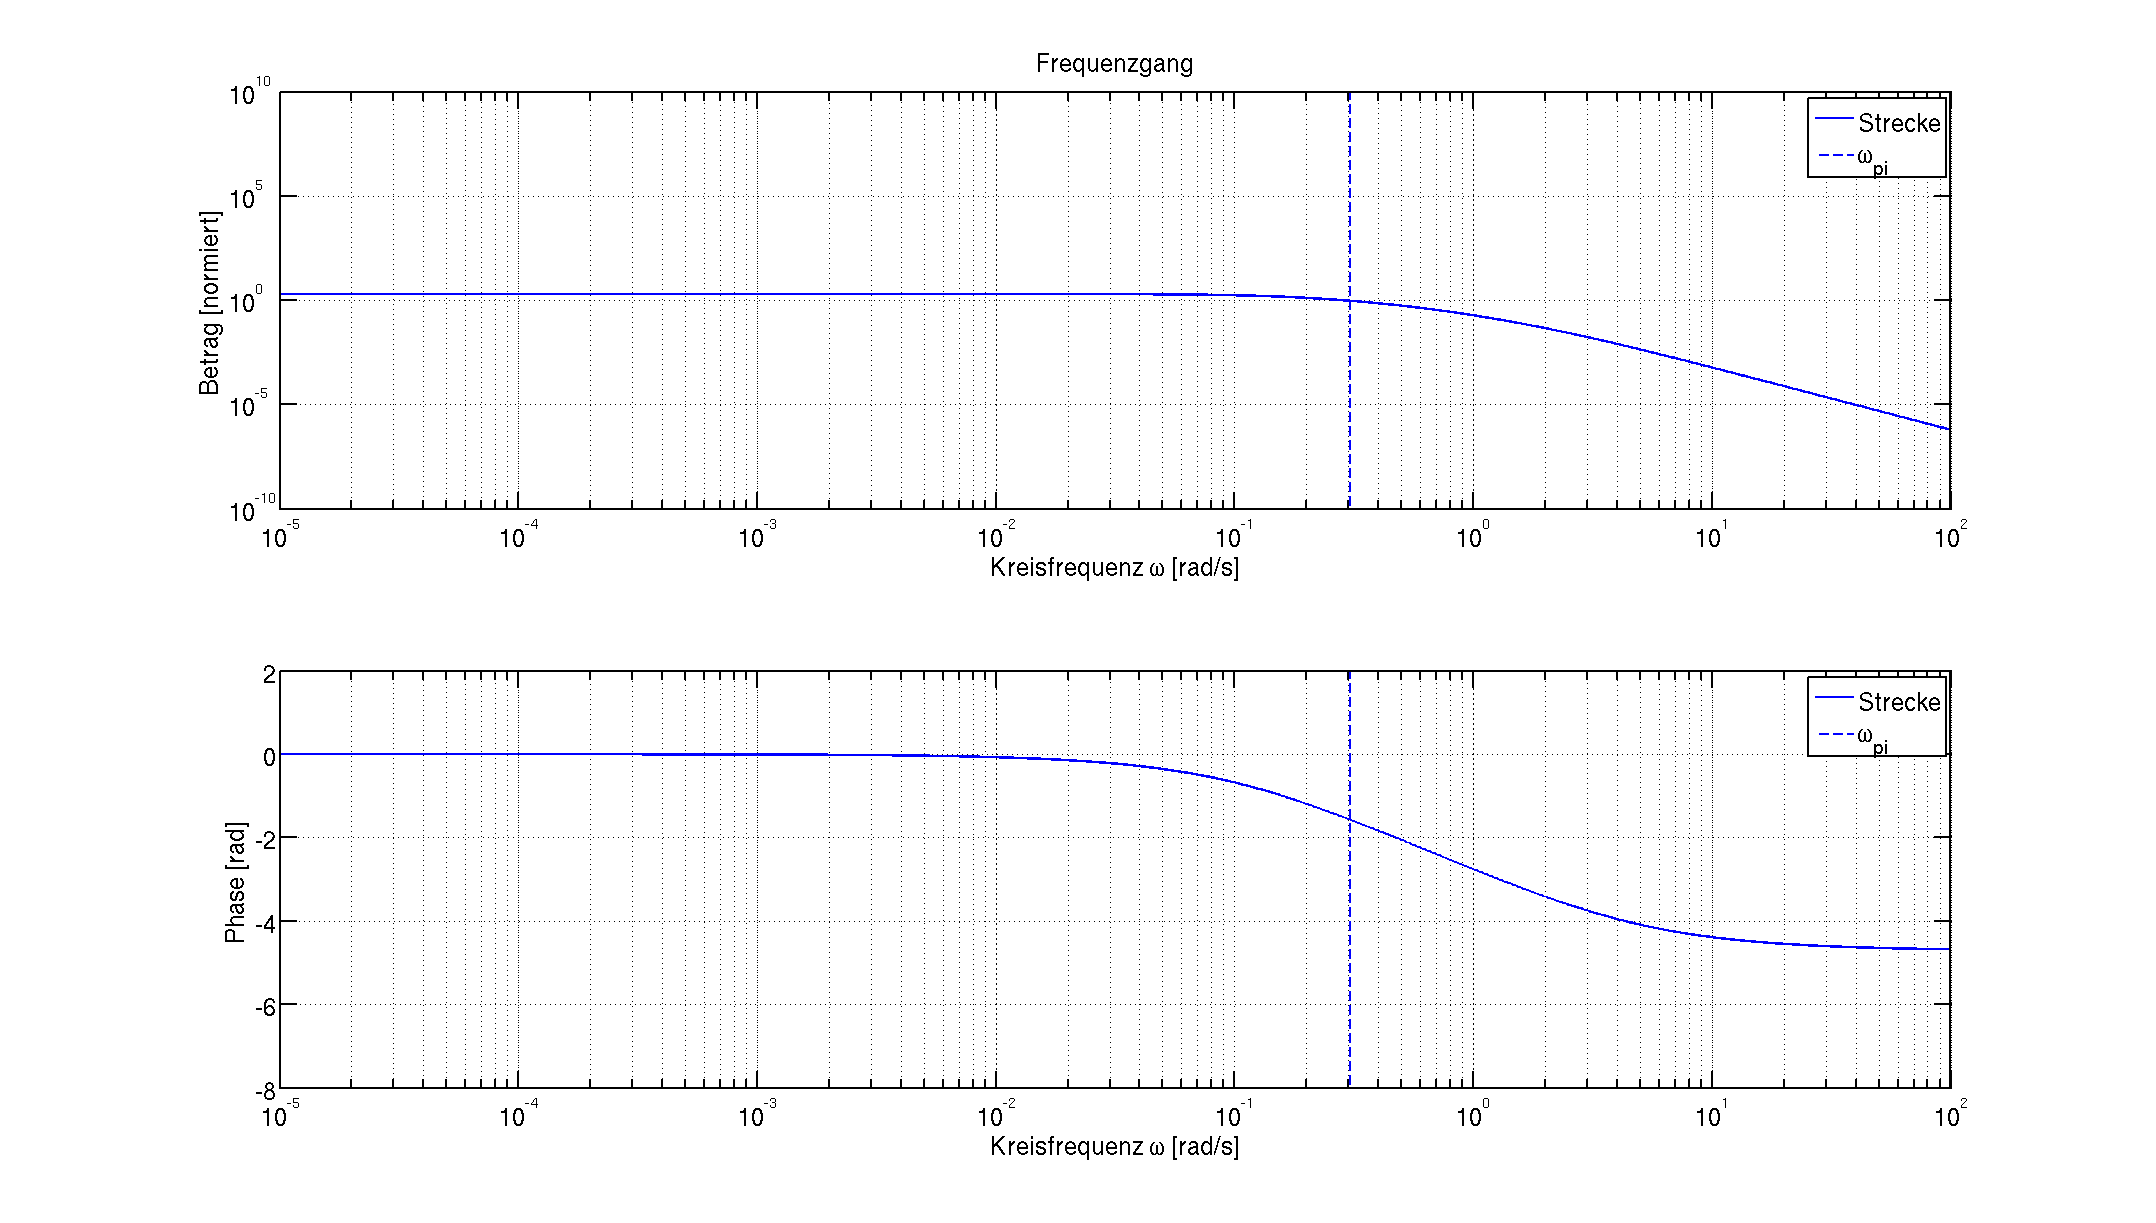
\includegraphics[width=\textwidth]{images/piStreckeOmegaPI.png}
    \caption{%
        Amplituden- und  Phasengang der Strecke mit  $\omega_{pi}$ eingetragen
        (vertikale gestrichelte Linie).
    }
    \label{fig:pi:omega_pi}
\end{figure}

Wie    man   aus    Abbildung~\ref{fig:pi:omega_pi}   ablesen    kann,   liegt
dieser   Wert  f\"ur   $\omega_{pi}$  in   unserem  Beispiel   bei  ungef\"ahr
$\SI{0.3}{\per\second}$. Die Kontrollrechnung mittels Matlab ergibt:

\begin{equation} \label{eq:pi:omega_pi}
    \omega_{pi} = \SI{0.3039}{\per\second}
\end{equation}


% ---------------------------------------------------------------------------- %
\subsubsection{Bestimmung von $\mathbf{T_{nk}}$}
% ---------------------------------------------------------------------------- %
Damit kann nun $T_{nk}$ direkt berechnet werden\footnotemark[5]:

\begin{equation} \label{eq:pi:omega_pi}
    T_{nk} = \frac{1}{\omega_{pi}} = \frac{1}{\SI{0.3039}{\per\second}} = \SI{3.2902}{\second}
\end{equation}

\footnotetext[5]{%
    Um die  Akkumulation von Ungenauigkeiten  zu minimieren, werden bei diesen
    Berechnungen  die  genauen  Werte  aus  Matlab  verwendet  und  nicht  die
    gerundeten  Zwischenresultate,  was  zu   Abweichungen  zu  den  von  Hand
    berechneten Ergebnissen f\"uhren kann.
}


% ---------------------------------------------------------------------------- %
\subsubsection{Bestimmung der Durchtrittsfrequenz $\mathbf{\boldsymbol{\omega}_d}$}
% ---------------------------------------------------------------------------- %

Die   Durchtrittsfrequenz  ist   die   Frequenz,  bei   der  die   betrachtete
\"Ubertragungsfunktion $H(j\omega)$ eine Verst\"arkung von $\SI{0}{\decibel} =
1$  aufweist. In der  Phasengangmethode soll  sie so  festgelegt werden,  dass
der  offene  Regelkreis  Gleichung~\ref{eq:phi_o} erf\"ullt. Dabei  ist  f\"ur
$\varphi_s$, abh\"angig vom gew\"unschten \"Uberschwingverhalten, ein Wert aus
Tabelle~\ref{tab:phi_s} auszuw\"ahlen\footnotemark[6].  Nach dem Festlegen der
Durchtrittsfrequenz (in  unserem Beispiel werden wir  $16.3\%$ anstreben) wird
dann im n\"achsten Abschnitt die Verst\"arkung des Reglers noch angepasst.

\footnotetext[6]{%
    Die  Werte f\"ur  $\varphi_s$  aus  Tabelle~\ref{tab:phi_s} stellen  keine
    abschliessende  Auflistung dar  und  sind lediglich  als Anhaltspunkte  zu
    betrachten. Weicht das Verhalten des geschlossenen Regelkreises am Schluss
    zu stark  vom gew\"unschten  Ergebnis ab, besteht  durch die  Wahl anderer
    Werte f\"ur $\varphi_s$ die M\"oglichkeit weiterer Optimierung.
}

\begin{equation} \label{eq:phi_o}
    \varphi_o(\omega_d)=\varphi_s.
\end{equation}

\begin{longtable}{llll}
    \toprule
    \endhead
    \endfoot
    \endlastfoot

    % CONTENT HERE ---------------------------------------------------------- %

    \"Uberschwingen & 0\%              & 16.3\%           & 23.3\% \\
    $\varphi_s$        & $-103.7 \degree$ & $-128.5 \degree$ & $-135 \degree$ \\

    \bottomrule
    \caption{Werte f\"ur $\varphi_s$}
    \label{tab:phi_s}
\end{longtable}

Um    Gleichung~\ref{eq:phi_o}    auswerten     zu    k\"onnen,    wird    der
Phasengang   des   offenen   Regelkreises   ben\"otigt. Dazu   wird   der   in
Gleichung~\ref{eq:pi:omega_pi}    erhaltene    Wert    f\"ur    $T_{nk}$    in
die   \"Ubertragungsfunktion    des   Reglers   (Gleichung~\ref{eq:pi:target})
eingesetzt. $K_{rk}$  ist  noch  unbekannt,  hat aber  auf  die  Phase  keinen
Einfluss und wird somit vorerst einfach auf 1 gesetzt.

\begin{gather} \label{eq:pi:target:inserted}
    \begin{split}
        H_{rpi} & = K_{rk} \cdot \biggl[ 1 + \frac{1}{s \cdot T_{nk}} \biggr] \\
                & = 1      \cdot \biggl[ 1 + \frac{1}{s \cdot \SI{3.2902}{\second}} \biggr]
    \end{split}
\end{gather}

Daraus kann nun der Frequenzgang  $H_o$ des offenen Regelkreises identifiziert
werden.

\begin{gather} \label{eq:pi:h_open}
    \begin{split}
        H_o (s) & = H_{rpi} (s) \cdot H_s (s) \\
            & = \Biggl(
                    K_{rk} \cdot \biggl[ 1 + \frac{1}{s \cdot T_{nk}} \biggr]
                \Biggr)
                \cdot
                K_s
                \cdot
                \Biggl(
                        \frac{1}{1 + s \cdot T_1}
                  \cdot \frac{1}{1 + s \cdot T_2}
                  \cdot \frac{1}{1 + s \cdot T_2}
                \Biggr) \\
            & = \Biggl(
                    1 \cdot \biggl[ 1 + \frac{1}{s \cdot \SI{3.2902}{\second}} \biggr]
                \Biggr)
                \cdot
                2
                \cdot
                \Biggl(
                          \frac{1}{1 + s \cdot \SI{0.4134}{\second}}
                    \cdot \frac{1}{1 + s \cdot \SI{1.4894}{\second}}
                    \cdot \frac{1}{1 + s \cdot \SI{5.3655}{\second}}
                \Biggr)
    \end{split}
\end{gather}


Von   besonderem    Interesse   ist   der    Phasengang   $\varphi_o(j\omega)$
dieser   \"Ubertragungsfunktion. Wie  oben   festgelegt,  soll   ein  maximals
\"Uberschwingen  von   ca. $16.3\%$  angestrebt  werden. Dazu   muss  gem\"ass
Tabelle~\ref{tab:phi_s}  die Durchtrittsfrequenz  $\omega_d$ gefunden  werden,
an  welcher der  offene  Regelkreis eine  Phase  von $-128.5\degree$  aufweist
(Gleichung~\ref{eq:phi_o}). In   Abbildung~\ref{fig:pi:omega_d}   kann   diese
Beziehung graphisch verifiziert werden.

\begin{figure}[h! width=\pagewidth]
    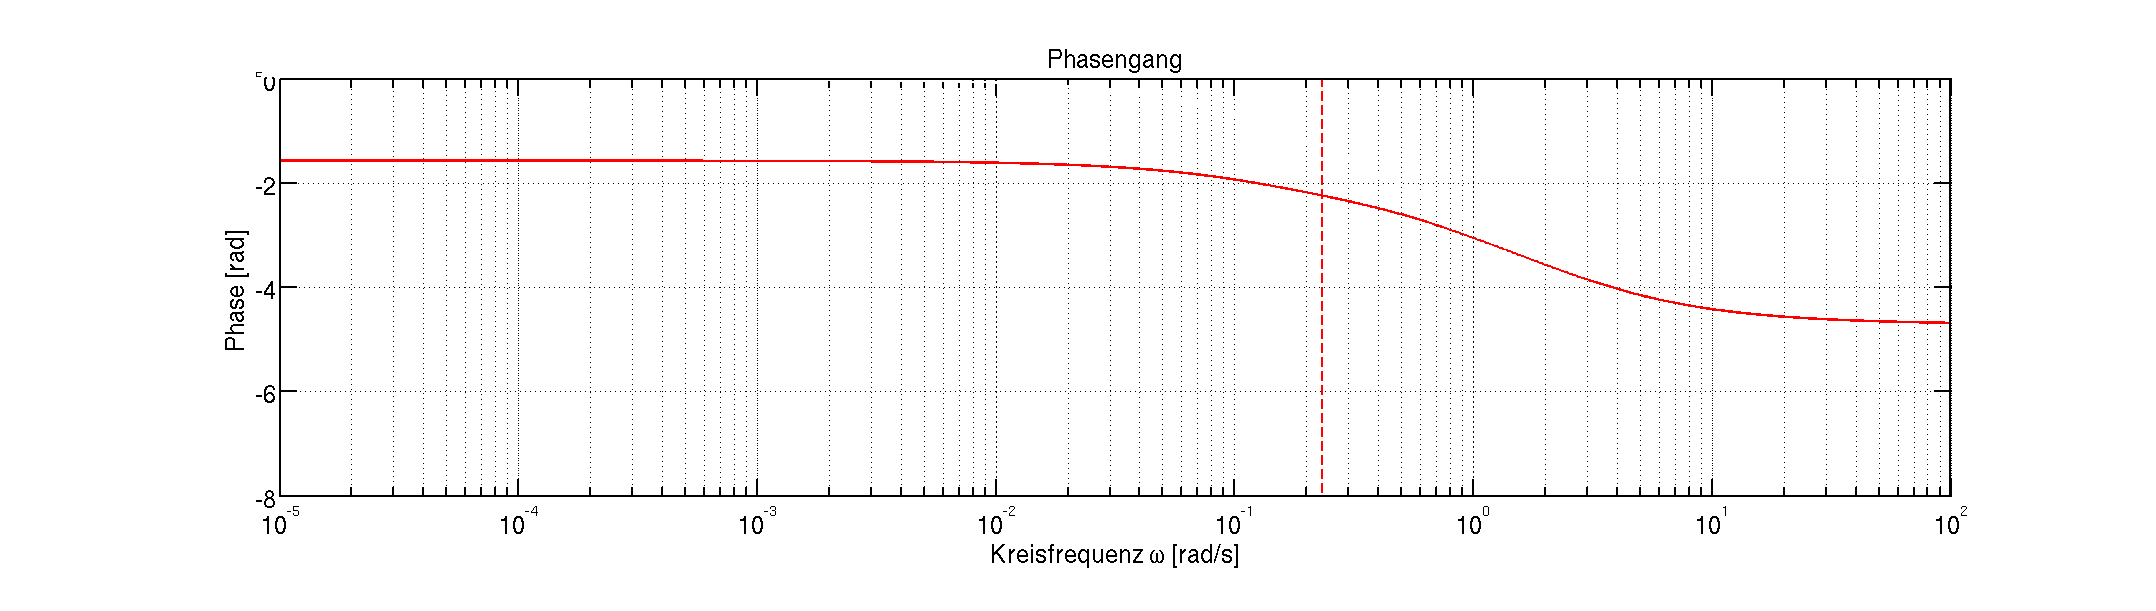
\includegraphics[width=\textwidth]{images/piOffenerRegelkreisPhasengang.png}
    \caption{%
        Phasengang   $\varphi_o(j\omega)$   des   offenen   Regelkreises   mit
        eingetragener Durchtrittsfrequenz $\omega_{d}$ (vertikale gestrichelte
        Linie). Wie man  sieht, weist der offene  Regelkreis unseres Beispiels
        bei dieser Kreisfrequenz eine Phase von $-128.5\degree$ auf
        (etwa $\SI{-2.24}{\radian}$).
    }
    \label{fig:pi:omega_d}
\end{figure}

Dies ergibt f\"ur die Durchtrittsfrequenz:
\begin{equation} \label{eq:pi:omega_d}
    \omega_d = \SI{0.2329}{\per\second}
\end{equation}


% ---------------------------------------------------------------------------- %
\subsubsection{Bestimmung der Reglerverst\"arkung $\mathbf{K_{rk}}$}
% ---------------------------------------------------------------------------- %

Im  letzten  Schritt  muss  nun, wie im  vorherigen  Abschnitt  erw\"ahnt, die
Verst\"arkung  $K_{rk}$   des  Reglers   noch  angepasst  werden,   damit  der
offene   Regelkreis  bei   der  angestrebten   Durchtrittsfrequenz  $\omega_d$
auch  effektiv  eine Verst\"arkung  von  1  aufweist.  Dazu  wird  $j\omega_d$
in  Gleichung~\ref{eq:pi:h_open}  f\"ur  den   Parameter  $s$  eingesetzt  und
$|H_o(j\omega_d)| = 1$ gesetzt.

\begin{gather} \label{eq:pi:A_o_set_to_one}
    \begin{split}
        A_o & = | H_o (j\omega_d) | = | H_{rpi} (j\omega) \cdot H_s (j\omega)| \\
            & = \abs*{
                    \bigg(
                        K_{rk} \cdot \biggl[ 1 + \frac{1}{j \cdot \omega_d \cdot T_{nk}} \biggr]
                    \bigg)
                    \cdot
                    K_s
                    \cdot
                    \bigg(
                            \frac{1}{1 + j \cdot \omega_d \cdot T_1}
                      \cdot \frac{1}{1 + j \cdot \omega_d \cdot T_2}
                      \cdot \frac{1}{1 + j \cdot \omega_d \cdot T_2}
                      \bigg)} \\
              & = 1
    \end{split}
\end{gather}

Mit den Werten
\begin{equation} \label{eq:pi:values}
    \begin{split}
        K_s      & = 2                    \\
        T_{nk}   & = \SI{3.2902}{\second} \\
        T_1      & = \SI{0.4134}{\second} \\
        T_2      & = \SI{1.4894}{\second} \\
        T_3      & = \SI{5.3655}{\second} \\
        \omega_d & = \SI{0.2329}{\radian\per\second}
    \end{split}
\end{equation}

l\"ost  man Gleichung  \ref{eq:pi:A_o_set_to_one}  nun nach  $K_{rk}$ auf  und
erh\"alt:

\begin{equation} \label{eq:pi:k_rk_result}
    K_{rk} = 0.517577
\end{equation}


% ---------------------------------------------------------------------------- %
\subsubsection{Resultat}
% ---------------------------------------------------------------------------- %

Somit ist der PI-Regler vollst\"andig bestimmt und hat folgende Form:

\begin{equation} \label{eq:pi:result}
    H_{rpi} = 0.518 \cdot \biggl[ 1 + \frac{1}{s \cdot \SI{3.29}{\second}} \biggr]
\end{equation}

In Abbildung~\ref{fig:pi:all} sind die  wichtigsten Werte f\"ur diesen Prozess
nochmals in einer \"Ubersicht zusammengefasst.

\begin{figure}[h! width=\pagewidth]
    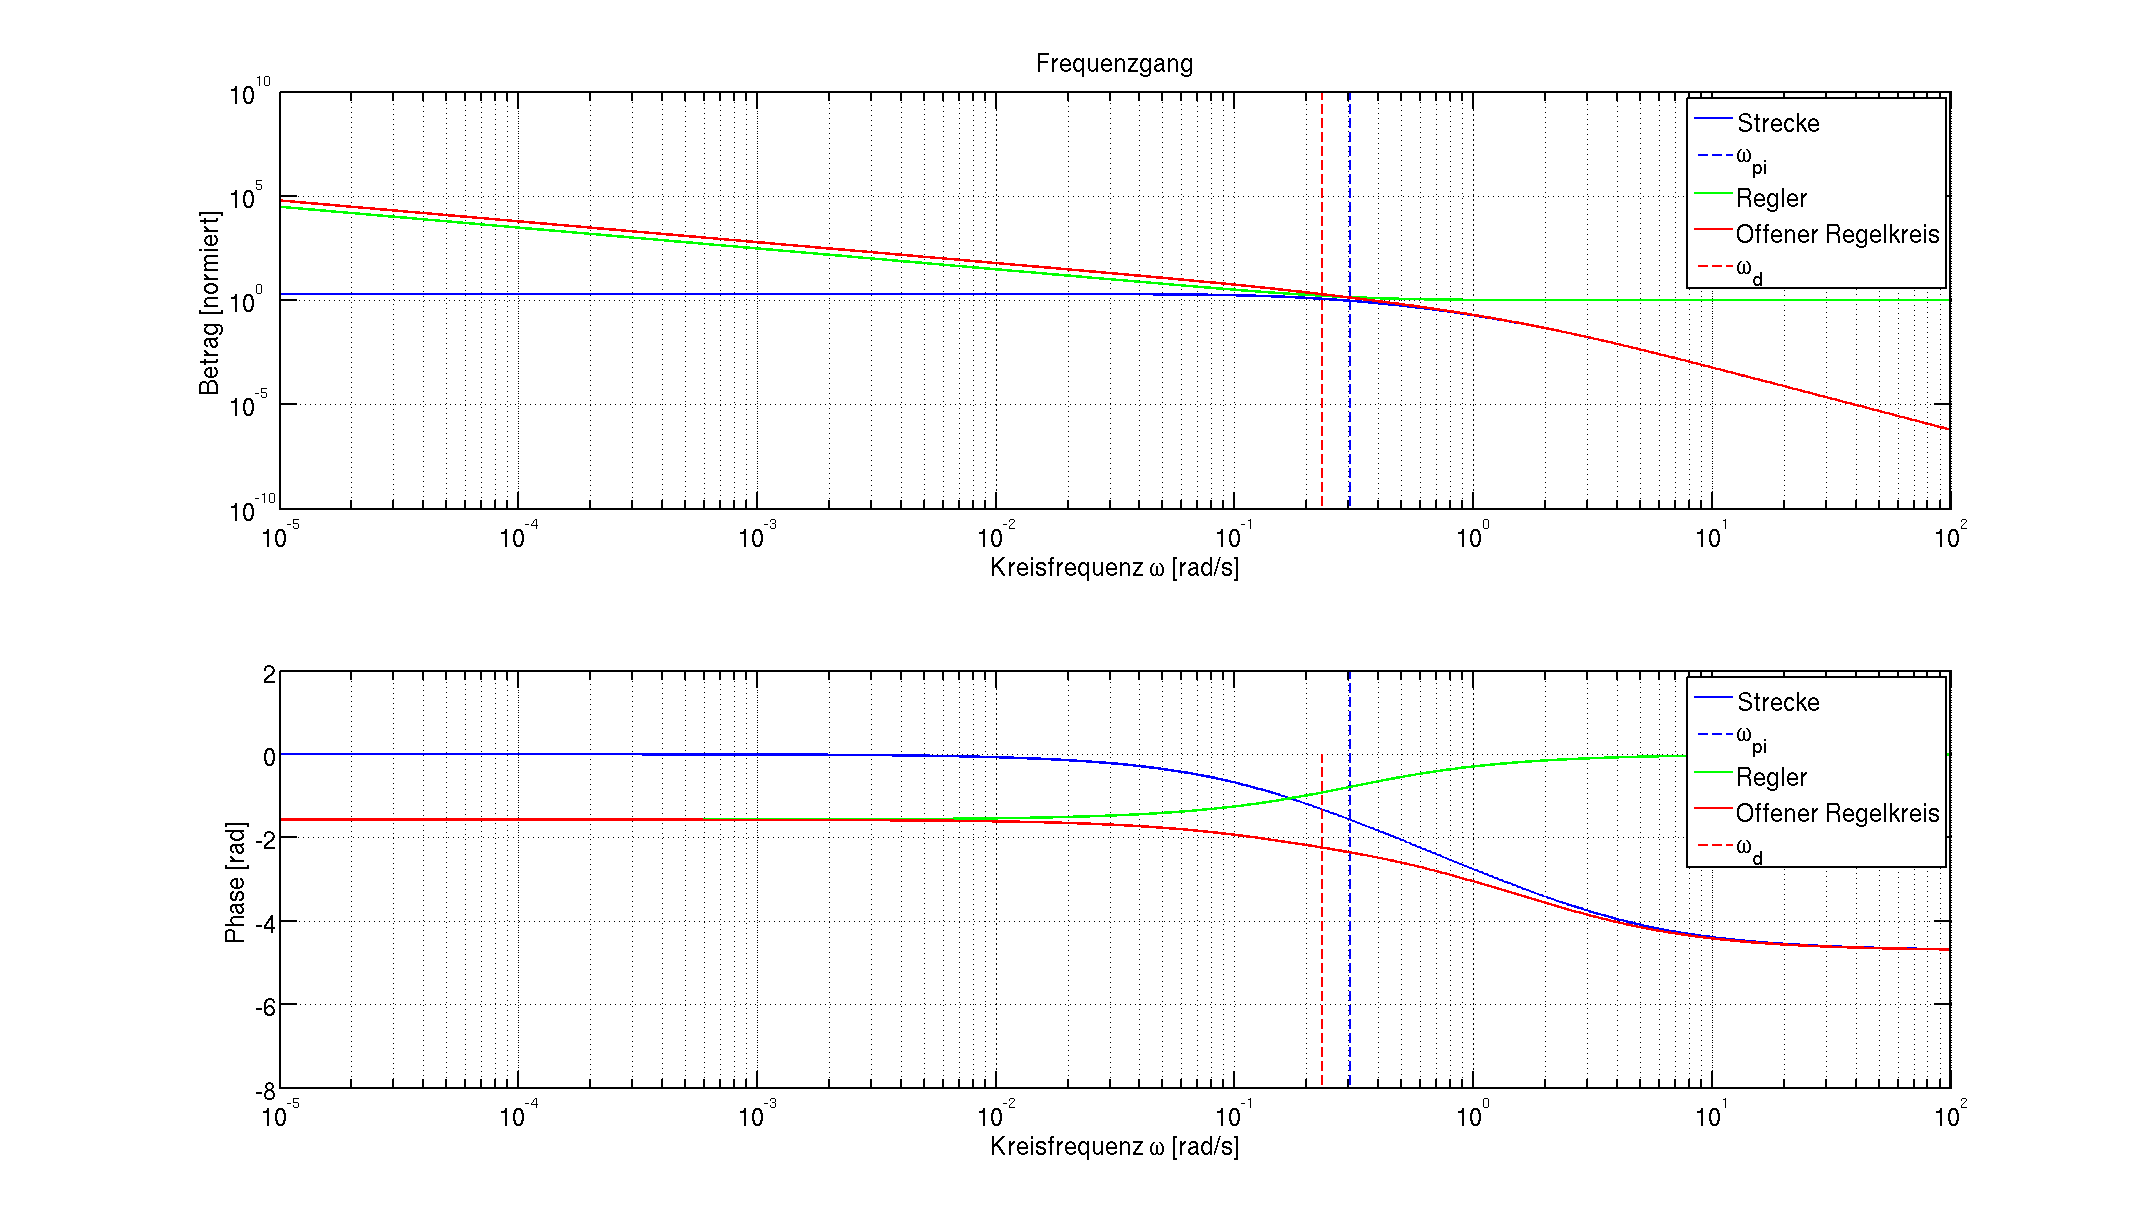
\includegraphics[width=\textwidth]{images/piBode.png}
    \caption{%
        Frequenzgang des Reglers (gr\"un), der  Strecke (blau) und des offenen
        Regelkreises (rot).
    }
    \label{fig:pi:all}
\end{figure}


\subsection{Reglerdimensionierung mittels Phasengangmethode: PID-Regler}
\label{subs:phasengang:pid}
\subsubsection*{Ziel}
Das Ziel ist  die Bestimmung der Parameter $K_{rk}$, $T_{nk}$  und $T_{vk}$ in
der Gleichung:

\begin{equation} \label{eq:pid:target}
    H_{rpid} = K_{rk} \cdot \biggl[ \frac{(1 + s \cdot T_{nk}) \cdot (1 + s \cdot T_{vk}) }{ s \cdot T_{nk} } \biggr]
\end{equation}


\subsubsection{Bestimmung der Reglerfrequenz $\omega_{pid}$}

Analog  zum PI-Regler  wird zuerst  im  Phasengang der  Strecke die  Frequenz
$\omega_{pid}$ bestimmt, f\"ur  welche die Phase der  Strecke einen bestimmten
Wert aufweist, nur wird hier $-135\degree$ benutzt:

\begin{equation} \label{eq:pid:phi_s}
    \varphi_s(\omega_{pid}) = -135 \degree
\end{equation}

In unserem Beispiel ergibt dies:

\begin{equation} \label{eq:pid:omega_pid}
    \omega_{pid} = \SI{0.6714}{\per\second}
\end{equation}


\subsubsection{Steigung des Phasengangs bei der Reglerfrequenz}

Anschliessend wird  die Steigung des  Phasengangs $\varphi_s$ der  Strecke bei
der  Frequenz  $\omega_{pid}$  bestimmt. Ausgangspunkt  daf\"ur  ist  die  von
\code{p\_sani} bestimmte  \"Ubertragungsfunktion der Strecke  (siehe Gleichung
\ref{eq:transfer:plant}).

\begin{equation} \label{eq:transfer:plant:derivative}
    \frac{d\varphi_s}{d\omega} \biggr \rvert_{\omega=\omega_{pid}}
        = \frac{d(arg(H_s(j\omega)))}{d\omega} \biggr \rvert_{\omega=\omega_{pid}}
        = \SI{-1.5124}{\second}
\end{equation}
\todo{Einheit \"uberpr\"ufen}


\subsubsection{Hilfsparameter $\beta$}

Zwischen den Steigungen der Phasen des offenen Regelkreises ($\varphi_o$), der
Strecke ($\varphi_s$) und des Reglers ($\varphi_r$) gilt folgende Beziehung:

\begin{equation} \label{eq:pid:phi_sum}
    \varphi_o = \varphi_s + \varphi_r
\end{equation}

Da die Ableitung eine lineare Funktion ist, gilt somit auch: \todo{korrekte Begriffe}
\begin{equation} \label{eq:pid:dphi_sum}
    \frac{d\varphi_o}{d\omega} = \frac{d\varphi_s}{d\omega} + \frac{d\varphi_r}{d\omega}
\end{equation}

Diese Beziehungen  k\"onnen auch  gut in Abbildung  \ref{fig:pid_complete} von
Hand \"uberpr\"uft werden.

Es soll nun gelten:

\begin{equation} \label{eq:pid:dphi_o_target}
    \frac{d\varphi_o}{d\omega} \biggr \rvert_{\omega=\omega_{pid}} = - \frac{1}{2}
\end{equation}

Da   $\frac{d\varphi_s}{d\omega}$  durch   die  Strecke   gegeben  und   somit
unver\"anderlich ist, kann lediglich der Wert von $\frac{d\varphi_r}{d\omega}$
angepasst     werden,     damit     $\frac{d\varphi_o}{d\omega}$     Gleichung
\ref{eq:pid:dphi_o_target} erf\"ullt.

Dazu f\"uhrt man den Hilfsparameter $\beta$ ein, f\"ur den gilt:

\begin{gather} \label{eq:pid:beta:start}
    \begin{split}
        \frac{1}{T_{vk}} & = \frac{\omega_{pid}}{\beta} \\
        \frac{1}{T_{nk}} & = \omega_{pid} \cdot \beta  \\
                       0 & <  \beta \leq 1
    \end{split}
\end{gather}

Die  beiden Frequenzen  $\frac{1}{T_{vk}}$  und  $\frac{1}{T_{nk}}$ sind  also
symmetrisch  um den  Faktor $\beta$  gr\"osser bzw.  kleiner als  die Frequenz
$\omega_{pid}$. \todo{siehe Plot} Will man  $\beta$ von Hand bestimmen, trifft
man zuerst eine ``vern\"unftige'' Annahme, zum Beispiel:

\begin{equation} \label{eq:pid:beta:initial_value}
    \beta = 0.5
\end{equation}

Mit  diesem Startwert  bestimmt  man nun  $T_{nk}$  und ${T_{vk}}$. Die  somit
erhaltenen Werte setzt man in  Gleichung \ref{eq:pid:target} ein, zusammen mit
dem Wert f\"ur $\omega_{pid}$ aus Gleichung \ref{eq:pid:omega_pid}:

\begin{gather} \label{eq:pid:t_nk_t_vk_initial_results}
    \begin{split}
        {T_{vk}} & = \frac{\beta}{\omega_{pid}}  = \frac{0.5}{\SI{0.6714}{\per\second}}                   = \SI{0.7447}{\second} \\
        {T_{nk}} & = \frac{1}{\omega_{pid} \cdot \beta} = \frac{1}{\SI{0.6714}{\per\second} \cdot 0.5 }  = \SI{2.9789}{\second} \\
    \end{split}
\end{gather}

Eingesetzt in die Reglergleichung, vorerst mit $K_{rk} = 1$:

\begin{gather} \label{eq:pid:t_nk_t_vk_initial_results}
    \begin{split}
        H_{rpid} & = K_{rk} \cdot \biggl[ \frac{(1 + j\omega \cdot T_{nk}) \cdot (1 + j\omega \cdot T_{vk}) }{ j\omega \cdot T_{nk} } \biggr] \\
                 & = 1      \cdot \biggl[ \frac{(1 + j\omega \cdot \SI{2.9789}{\second}) \cdot (1 + j\omega \cdot \SI{0.7447}{\second}) }{ j\omega \cdot  \SI{2.9789}{\second}} \biggr]
    \end{split}
\end{gather}

Von dieser Gleichung bestimmt man nun den Phasengang und wertet danach dessen
Ableitung an der Stelle $\omega = \omega_{pid}$ aus:

\begin{gather} \label{eq:pid:phi_r_first_iteration}
    \begin{split}
        \varphi_s (j\omega)                                            & = arg(H_{rpid}(j\omega))        \\
        \frac{d\varphi_s}{d\omega} \biggr \rvert_{\omega=\omega_{pid}} & = \SI{1.1920}{\second}
    \end{split}
\end{gather}
\todo{Die zugeh\"orige Rechnung ist lange und m\"uhsam, allenfalls in Anhang? Ebenfalls: Einheit kontrollieren}


Setzt man dies in Gleichung \ref{eq:pid:phi_sum} ein, erh\"alt man:
\begin{gather} \label{eq:pid:phi_sum_result_iteration_one}
    \begin{split}
    \frac{d\varphi_o}{d\omega}       \biggr \rvert_{\omega=\omega_{pid}, \beta=0.5}
        & = \frac{d\varphi_s}{d\omega} \biggr \rvert_{\omega=\omega_{pid}}
        + \frac{d\varphi_r}{d\omega} \biggr \rvert_{\omega=\omega_{pid}, \beta=0.5} \\
        & = \SI{-1.5124}{\second} + \SI{1.1920}{\second} \\
        & = \SI{-0.3204}{\second} \\
        & > -\frac{1}{2}
    \end{split}
\end{gather}

Mit  $\beta  = 0.5$  erh\"alt  man  also eine  zu  hohe  Steigung des  offenen
Regelkreises   an    der   Stelle  $\omega_{pid}$,   folglich   muss   $\beta$
{\em{verkleinert}} werden.   Diese Berechnungen  werden nun mit  jeweils neuen
Werten  f\"ur  $\beta$  solange  wiederholt,  bis  die  Steigung  des  offenen
Regelkreises die gew\"unschte N\"ahe zu $-\frac{1}{2}$ aufweist.

Da die manuelle Iterierung dieses Prozesses enorm viel Zeit in Anspruch nimmt,
bietet  sich  hier  eine  Automatisierung  an. Die  Berechnung  mittels  eines
geeigneten Algorithmus in Matlab liefert schlussendlich folgendes Ergebnis:
\todo{Allenfalls Matlab-Algo in Anhang und Verweis}

\begin{gather} \label{eq:pid:beta_result}
    \begin{split}
        \beta    & = 0.2776 \\
        {T_{vk}} & = \frac{\beta}{\omega_{pid}}           = \SI{0.4134}{\second} \\
        {T_{nk}} & = \frac{1}{\omega_{pid} \cdot \beta}   = \SI{5.3656}{\second} \\
    \end{split}
\end{gather}

Sollte  man  f\"ur  $\beta$  einen komplexen  Wert  erhalten,  wird  $\beta=1$
gesetzt.\todo{Wie kann dies egtl. passieren?}


\subsubsection{Durchtrittsfrequenz $\omega_d$}

Diese  Werte setzt man nun in Gleichung \ref{eq:pid:target} ein. $K_{rk}$ wird
wie bei der Bestimmung von $\beta$ vorerst noch auf 1 gesetzt.

\begin{gather} \label{eq:pid:h_rpid_beta_result}
    \begin{split}
        H_{rpid} & = K_{rk} \cdot \biggl[ \frac{(1 + s \cdot T_{nk}               ) \cdot (1 + s \cdot T_{vk}               ) }{ s \cdot T_{nk}               } \biggr]
                   = 1      \cdot \biggl[ \frac{(1 + s \cdot \SI{5.3656}{\second} ) \cdot (1 + s \cdot \SI{0.4134}{\second} ) }{ s \cdot \SI{5.3656}{\second} } \biggr]
    \end{split}
\end{gather}

Zur Bestimmung von $K_{rk}$ wird nun der Frequenzgang des offenen Regelkreises
betrachtet. Dazu  multipliziert  man  wie  gehabt  die  \"Ubertragungsfunktion
der  Strecke   (siehe  Gleichung   \ref{eq:transfer:plant})  mit   der  soeben
bestimmten  provisorischen   \"Ubertragungsfunktion  des   Reglers  (Gleichung
\ref{eq:pid:h_rpid_beta_result}).

\begin{equation} \label{eq:pid:h_o_k_rk_one}
    H_{o}(j\omega) = H_{rpid}(j\omega) \cdot H_s(j\omega)
\end{equation}

Nun wird  die Durchtrittsfrequenz $\omega_d$  bestimmt, an welcher  der offene
Regelkreis eine  Verst\"arkung von $\SI{0}{\decibel} =  1$ aufweisen soll. Wie
auch  beim  PI-Regler  werden  wir   hier  ein  \"Uberschwingen  von  $16.3\%$
anstreben, womit gem\"ass Tabelle \ref{tab:phi_s}gilt:

\begin{equation} \label{eq:pid:omega_d_target}
    \varphi_s(\omega_d) = \varphi_s = -128.5\degree
\end{equation}

Dieser Wert wird analog zum PI-Regler aus dem Phasengang des offenen Regelkreises
abgelesen. \todo{siehe Plot} Eine Nachrechnung mittels Matlab ergibt:


\begin{equation} \label{eq:pid:omega_d_target}
    \omega_d = \SI{0.5341}{\per\second}
\end{equation}


\subsubsection{Bestimmung der Reglerverst\"arkung $K_{rk}$}

In einem letzten Schritt wird  nun der Amplitudengang des offenen Regelkreises
an der  Stelle $\omega_d$ gleich 1  gesetzt und diese Gleichung  nach $K_{rk}$
aufgel\"ost:

\begin{equation} \label{eq:pid:h_o_k_rk_one}
    \begin{split}
        A_{o}(j\omega_d)    & = | H_{o}(j\omega_d) |                            \\
                            & = | H_{rpid}(j\omega_d) \cdot H_s(j\omega_d) |    \\
                            & = \Biggl \rvert
                                    K_{rk}
                                    \cdot
                                    \biggl[ \frac{(1 + j\omega_d \cdot T_{nk}) \cdot (1 + j\omega_d \cdot T_{vk}) }{ j\omega_d \cdot T_{nk} } \biggr] \Biggr \rvert \\
                            & \cdot
                                \Biggl \rvert
                                    K_s
                                    \cdot \frac{1}{1 + j\omega_d \cdot T_1}
                                    \cdot \frac{1}{1 + j\omega_d \cdot T_2}
                                    \cdot \frac{1}{1 + j\omega_d \cdot T_2}
                                    \Biggr \rvert \\
                            & = 1
    \end{split}
\end{equation}

Mit den gegebenen und berechneten Werten:
\begin{gather} \label{eq:pid:h_o_k_rk_one}
    \begin{split}
        K_s         & = 2                        \\
        T_1         & = \SI{0.4134}{\second}     \\
        T_2         & = \SI{1.4894}{\second}     \\
        T_3         & = \SI{5.3655}{\second}     \\
        T_{nk}      & = \SI{5.3656}{\second}     \\
        T_{vk}      & = \SI{0.4134}{\second}     \\
        \omega_d    & = \SI{0.5341}{\per\second}
    \end{split}
\end{gather}

Dies liefert:

\begin{equation} \label{eq:pid:k_rk_result}
    K_{rk} = 1.83084
\end{equation}


\subsubsection{Resultat}

Somit ist der Regler vollst\"andig bestimmt und hat folgende \"Ubertragungsfunktion:

\begin{equation} \label{eq:pid:result}
    H_{rpid}(s) = 1.83084 \cdot \biggl[ \frac{(1 + s \cdot \SI{5.3656}{\second} ) \cdot (1 + s \cdot \SI{0.4134}{\second} ) }{ s \cdot \SI{5.3656}{\second} } \biggr]
\end{equation}

Die Frequenzg\"ange der Strecke, des Reglers und des offenen Regelkreises:

\begin{figure}[h! width=\pagewidth]
    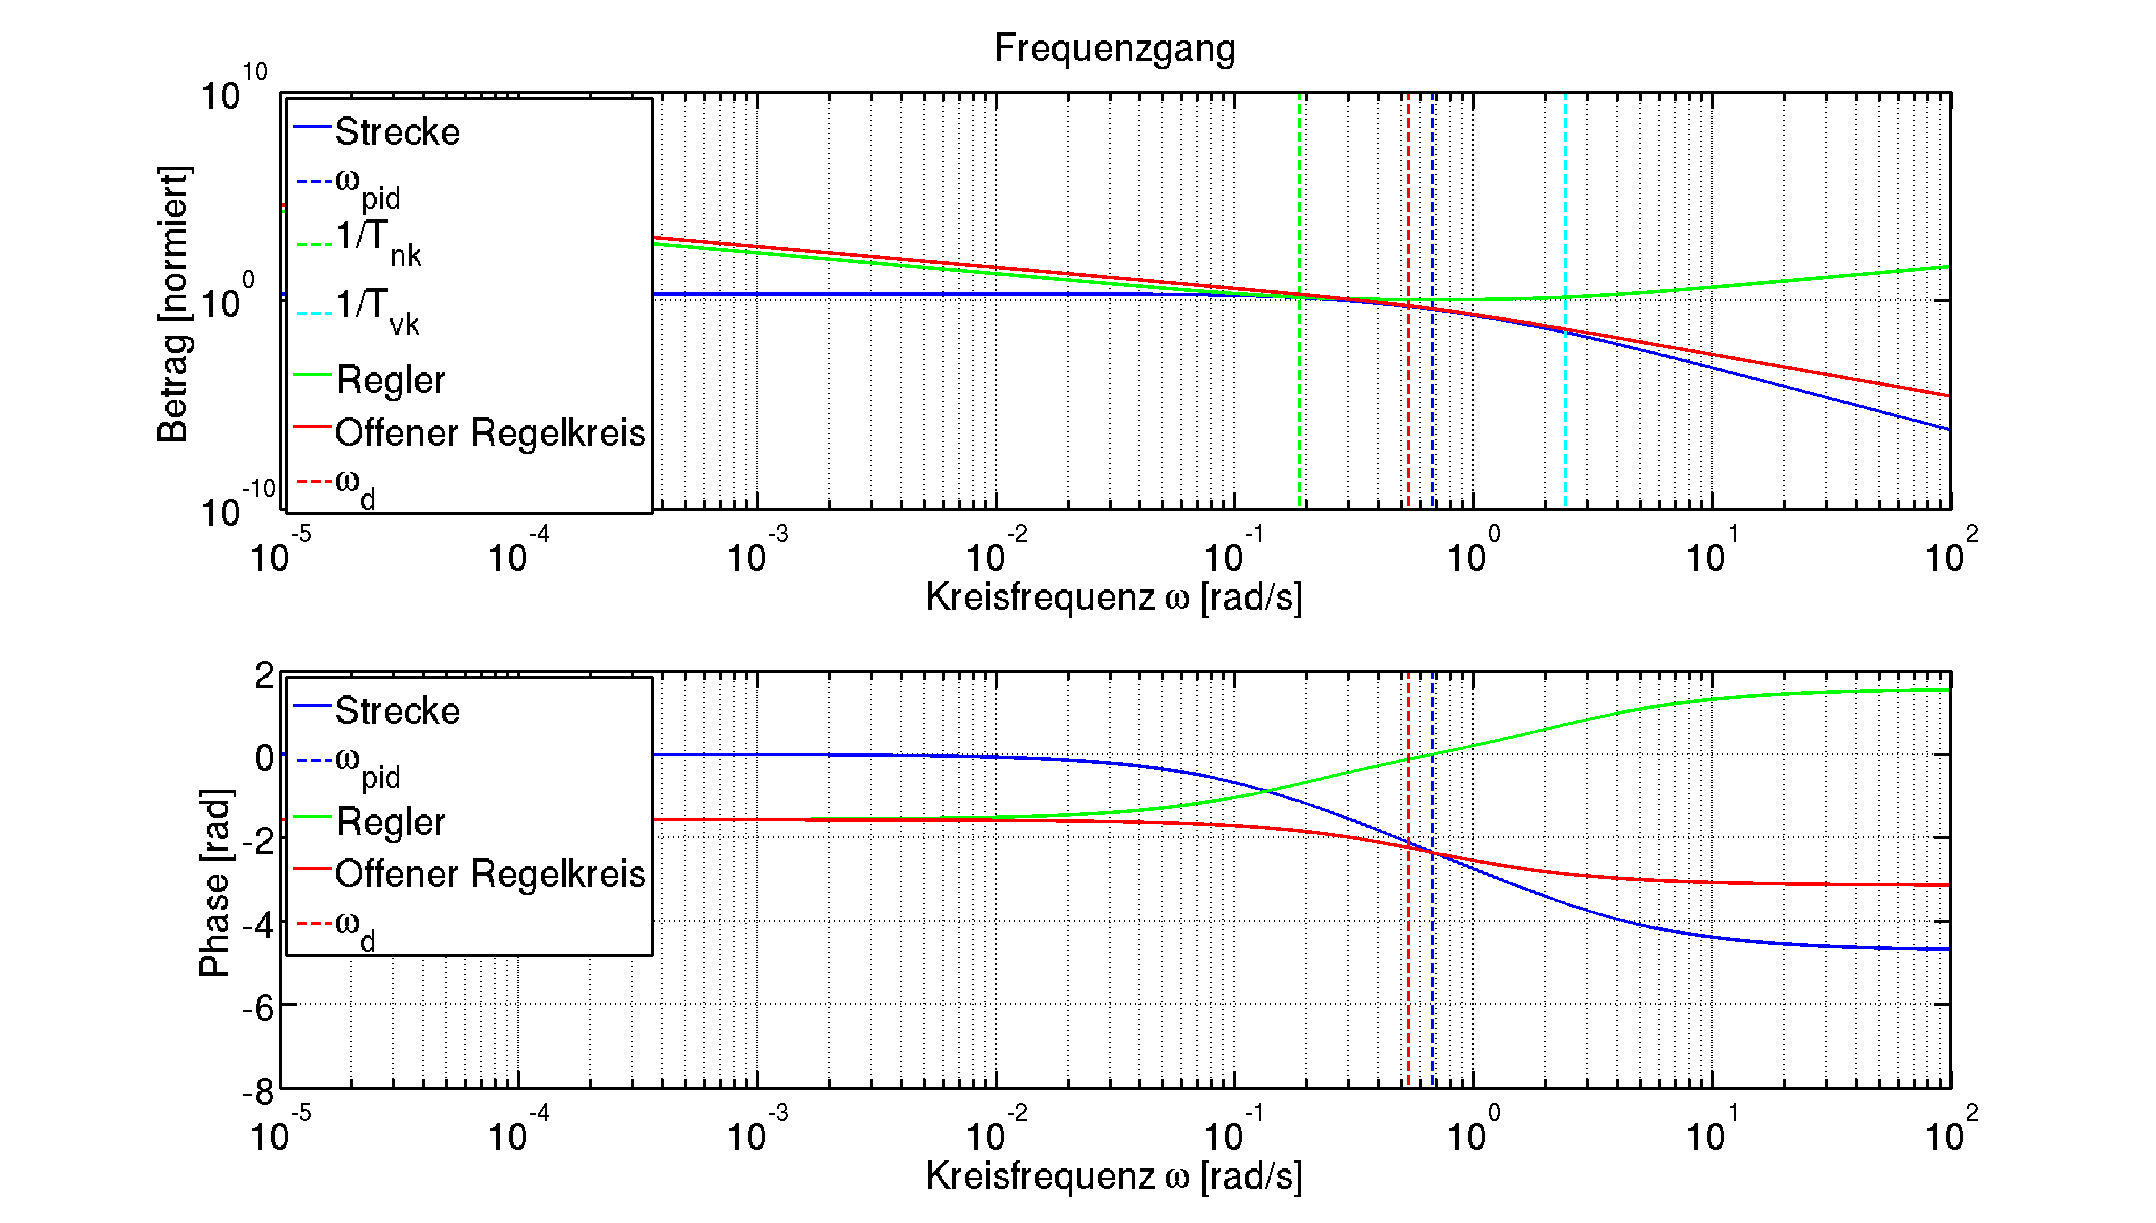
\includegraphics[width=\textwidth]{images/pidCompletePlot.png}
    \caption{%
        Frequenzgang der Strecke (blau), des  Reglers (gr\"un) und des offenen
        Regelkreises  (rot).  Ebenfalls  eingetragen  sind die  Reglerfrequenz
        $\omega_{pid}$,   die   beiden   Frequenzen   $\frac{1}{T_{vk}}$   und
        $\frac{1}{T_{nk}}$ sowie die Durchtrittsfrequenz $\omega_d$.
    }
    \label{fig:pid_complete}
\end{figure}
\clearpage


\subsection{Umrechnung zwischen bodekonformer und reglerkonformer Darstellung}
\label{subs:bode_regler}
Ein Regler  kann mittels verschiedener mathematischen  Gleichungen dargestellt
werden.  F\"ur  die Berechnungen  in diesem Projekt  sind zwei  von besonderer
Bedeutung: Die bodekonforme und die reglerkonforme Darstellung.

Dabei gilt  es zu  beachten, dass  sich die  einzelnen Darstellungen  in ihrer
mathematischen Gleichung  unterscheiden, jedoch den  selben Informationsinhalt
haben. Deshalb   ist  es   auch  m\"oglich,  mittels  einfacher   Umrechnungen
die  Darstellungsweise   zu  wechseln.

Der  Grund,   weshalb  zwei  verschiedene  Darstellungsarten   existieren  und
verwendet werden, liegt zum einen darin, dass gewisse Berechnungen automatisch
die eine oder andere Darstellungsart  zur\"uckgeben, jedoch auch, dass je nach
Situation der  Verst\"andlichkeit halber die eine  oder andere Darstellungsart
bevorzugt wird.

Bei der  bodekonformen Darstellung wie  in Gleichungen~\ref{eq:pi:bodekonform}
und~\ref{eq:pid:bodekonform}   ist   die  \"Ubertragungsfunktion   leicht   zu
interpretieren,  was ihren  Amplitduden- und  Frequenzgang betrifft.   Deshalb
wird  die  bodekonforme  Darstellung  \"uberall dort  verwendet,  wo  mit  den
Reglerwerten Berechnungen ausgef\"uhrt werden.

\begin{equation} \label{eq:pi:bodekonform}
    H_{rpi} = K_{rk} \cdot \biggl[ \frac{1 + s \cdot T_{nk}}{s \cdot T_{nk}} \biggr]
\end{equation}

\begin{equation} \label{eq:pid:bodekonform}
    H_{rpid} = K_{rk} \cdot \biggl[ \frac{(1 + s \cdot T_{nk}) \cdot (1 + s \cdot T_{vk}) }{ s \cdot T_{nk} } \biggr]
\end{equation}


Die reglerkonforme  Darstellung aus  den Gleichungen~\ref{eq:pi:reglerkonform}
und~\ref{eq:pid:reglerkonform}  hingegen ist  so  aufgebaut,  dass die  Werte,
welche  an  einem realen  Regler  einstellbar  sind, direkt  abgelesen  werden
k\"onnen. Diese Darstellung  wird verwendet,  um die Reglerwerte  dem Benutzer
zur Verf\"ugung zu stellen.

\begin{equation} \label{eq:pi:reglerkonform}
    H_{rpi} = K_{r} \cdot \biggl[ 1 + \frac{1}{s \cdot T_{n}} \biggr]
\end{equation}

\begin{equation} \label{eq:pid:reglerkonform}
    H_{rpid} = K_{r} \cdot \biggl[ 1 + \frac{1}{s \cdot T_n} + \frac{s \cdot T_v}{s \cdot T_p} \biggr]
\end{equation}

Zudem   liegt   das   Ergebnis   der    Faustformeln   auch   immer   in   der
reglerkonformen  Darstellung  vor. F\"ur  die  Umrechnung  zwischen  den  zwei
Darstellungsarten  ergibt  sich  durch  einen  Koeffizientenvergleich  Tabelle

\ref{tab:bode_regler_konform}.

\begin{longtable}{l|ll}
    \toprule

    %\multicolumn{3}{l}{\large{\textsc{auftragsanalyse und hintergrundinformationen}}} \\
    %\multicolumn{2}{l}{pi}

    &
    bodekonform $\rightarrow$ reglerkonform
    &
    reglerkonform $\rightarrow$ bodekonform
    \\

    \midrule

    \endhead
    \endfoot
    \endlastfoot

    % content here ---------------------------------------------------------- %

    PI
    &
    $T_n = T_{nk} $ %reglerkonform
    &
    $K_{rk} = K_r $ %bodekonform
    \\

    \midrule

    PID
    &
    $T_n = T_{nk}+T_{vk}-T_p$
    &
    $T_{nk}=0.5 \cdot (T_n+T_p) \cdot (1+\epsilon)$
    \\

    &
    $T_v=\frac{T_{nk} \cdot T_{vk}}{T_{nk}+T_{vk}-T_p}-T_p$
    &
    $T_{vk}=0.5 \cdot (T_n+t_p) \cdot (1-\epsilon)$
    \\

    &
    %$k_r=k_{rk} \cdot \frac{1+t_{vk}}{t_{nk}}$
    $K_r=K_{rk} \cdot (1 + \frac{T_{vk}-T_p}{T_{nk}})$
    &
    $K_{rk} = 0.5 \cdot K_r \cdot (1 + \frac{T_p}{T_{nk}}) \cdot (1+\epsilon )$
    \\
    \\

    &
    \multicolumn{2}{l}{wobei $\epsilon^2 = 1-(4 \cdot T_n \cdot \frac{T_v-T_p}{(T_n+T_p)^2})$}
    \\
    \bottomrule
    \caption{Formeln zur Umrechung zwischen bode- zu reglerkonformer Darstellung \cite{regelungstechnik:zellweger}, \cite{regelungstechnik:schumleon}}
    \label{tab:bode_regler_konform}
\end{longtable}


F\"ur die Berechnungen in diesem Projekt wird, wenn nicht anders angegeben, mit $T_p=\frac{1}{10} \cdot T_v$ gerechnet.


\subsection{Schrittantwort des geschlossenen Regelkreises}
Die    Aufgabe   eines    geschlossenen    Regelkreises (Abbildung \ref{fig:geschlossenerRegelkreis}) ist  es, einen  vorgegeben Sollwert  zu erreichen  und diesen
auch bei  St\"orungen aufrecht zu  erhalten. Dabei sollen die  unten genannten
dynamischen  Anforderungen  eingehalten  werden, damit  die  Stabilit\"at  des
Regelsystems garaniert ist. Die wichtigste  Bedingung f\"ur die Schrittantwort
ein  geschlossenen  Regelkreis heisst,  dass  der  Regelfehler, die  Differenz
zwischen Ist-und Sollwert, gleich Null oder m\"oglichst klein ist.\\


\begin{figure}[!h!, width=\pagewidth]
\begin{center}
    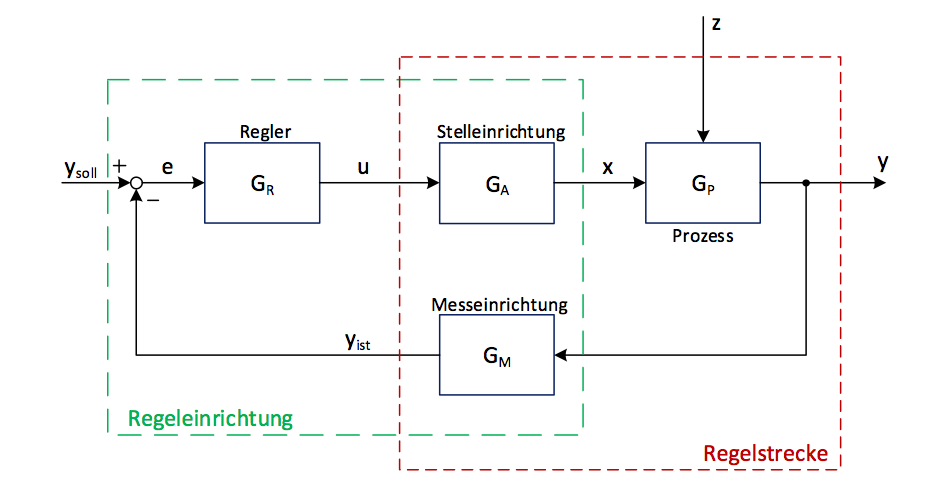
\includegraphics[width=0.5\textwidth]{images/geschlRegelkreis}
    \caption{Geschlossener Regelkreis}
    \label{fig:geschlossenerRegelkreis}
\end{center}
\end{figure}

%Name Bild Struktur eines allgemeinen Regelkreises
\begin{itemize}
    \item
        $y_soll$ bezeichnet den Sollwert der Regelgr\"osse.
    \item
        $e$ Regelabweichung (Regelfehler)
    \item
        $u$ Steuergr\"osse
    \item
        $x$ Stellgr\"osse
    \item
        $y$ Regelgr\"osse
    \item
        $z$ St\"orgr\"osse
    \item
        $y_ist$  ist der  Ist-Wert der  Regelgr\"osse  und wird  auch als  die
        Schrittantwort des Regelkreis bezeichnet.
\end{itemize}

\todo{Bild Schrittantworten passend zu Aufzählung unten}

Grunds\"atzlich  k\"onnen  f\"unf   Anforderungen  f\"ur  einen  geschlossenen
Regelkreis und deren Schrittantworten zusammengefasst werden:\\
\begin{enumerate}
    \item Der Regelkreis muss stabil sein:
        \begin{itemize}
            \item
                Das heisst  f\"ur die Schrittantwort, dass  nach dem Erreichen
                des  eingeschwungenen  Zustand kein  erneutes  \"Uberschwingen
                stattfinden darf.
            \item
                F\"ur  das  Regelsystem  heisst  stabil,  dass  es  in  seinen
                Gleichgewichtszustand zur\"uckgef\"uhrt werden kann.
        \end{itemize}
    \item
        Der Regelkreis  muss gen\"ugend ged\"ampft sein: \\Die  D\"ampfung der
        Schrittantwort soll  so stark  sein, dass der  eingeschwungene Zustand
        m\"oglichst  rasch erreicht  wird  ohne dass  das \"Uberschwingen  des
        Systems zu stark wird.
    \item
        Der   Regelkreis   muss   eine  bestimmte   station\"are   Genauigkeit
        aufweisen: Das  bedeutet,  der  Regelfehler  e(t) soll  f\"ur  t->  oo
        gegen  Null  gehen. F\"ur  die  Schrittantwort heisst  das,  dass  die
        Schrittantwort gleich $y_soll$ sein muss.
    \item
        Der Regelkreis  muss hinreichend  schnell sein: Die  Schnelligkeit des
        Einschwingvorganges der  Schrittantwort ist  stark von  der D\"ampfung
        abh\"angig. Ist die D\"ampfung  zu stark oder zu  schwach, braucht der
        Einschwingvorgang mehr Zeit. Hierbei muss darauf geachtet werden, dass
        die spezifischen Anforderungen an das Regelsystem eingehalten werden.
    \item
        Der  Regelkreis muss  robust  sein: Der Regelkreis  muss so  ausgelegt
        werden,  dass  das  Regelsystem  auch im  schlimmsten  Fall  (je  nach
        Regelsystem situationsabh\"angig) in der Lage ist, das System zur\"uck
        in den stabilen Zustand (vgl. 1.) zu regeln.
\end{enumerate}

